\documentclass[article,shortnames]{jss}

%% -- LaTeX packages and custom commands ---------------------------------------

%% recommended packages
\usepackage{thumbpdf,lmodern}

%% additional packages
\usepackage{amssymb,amsmath}

%% new custom commands
\newcommand{\class}[1]{`\code{#1}'}
\newcommand{\fct}[1]{\code{#1()}}

%% For Sweave-based articles about R packages:
%% need no \usepackage{Sweave}



%% -- Article metainformation (author, title, ...) -----------------------------

%% - \author{} with primary affiliation
%% - \Plainauthor{} without affiliations
%% - Separate authors by \And or \AND (in \author) or by comma (in \Plainauthor).
%% - \AND starts a new line, \And does not.
\author{Lennart Oelschl\"ager \\Bielefeld University \And Dietmar Bauer\\Bielefeld University}
\Plainauthor{Lennart Oelschl\"ager, Dietmar Bauer}

%% - \title{} in title case
%% - \Plaintitle{} without LaTeX markup (if any)
%% - \Shorttitle{} with LaTeX markup (if any), used as running title
\title{\pkg{RprobitB}: Bayes Estimation of Choice Behavior Heterogeneity in \proglang{R}}
\Plaintitle{RprobitB: Bayes Estimation of Choice Behavior Heterogeneity in R}
\Shorttitle{RprobitB}

%% - \Abstract{} almost as usual
\Abstract{
\pkg{RprobitB} is an \proglang{R} package for Bayes estimation of probit choice models, both in the cross-sectional and panel setting. The package analyses binary, multivariate, ordered, or ranked choices, and has a special focus on modeling choice behavior heterogeneity among deciders. The main functionality includes model fitting via Markov chain Monte Carlo methods, tools for convergence diagnostic, choice data simulation, in-sample and out-of-sample choice prediction, and model selection on the basis of information criteria and Bayes factors. The package facilitates preference-based decider classification via the latent class model extension, where the underlying class number can be inferred using the Dirichlet process or a weight-based updating scheme.
}

%% - \Keywords{} with LaTeX markup, at least one required
%% - \Plainkeywords{} without LaTeX markup (if necessary)
%% - Should be comma-separated and in sentence case.
\Keywords{discrete choice, probit model, choice behavior heterogeneity, Bayes estimation, decider classification, \proglang{R}}
\Plainkeywords{discrete choice, probit model, choice behavior heterogeneity, Bayes estimation, decider classification, R}

%% - \Address{} of at least one author
%% - May contain multiple affiliations for each author
%%   (in extra lines, separated by \emph{and}\\).
%% - May contain multiple authors for the same affiliation
%%   (in the same first line, separated by comma).
\Address{
  Lennart Oelschl\"ager, Dietmar Bauer\\
  Department of Business Administration and Economics\\
  Bielefeld University\\
  Postfach 10 01 31\\
  E-mail: \email{lennart.oelschlaeger@uni-bielefeld.de}, \email{dietmar.bauer@uni-bielefeld.de}
}

\begin{document}
%% I have no idea what this does. Maybe we need this in the future.
%% \SweaveOpts{concordance=TRUE}

%% -- Introduction -------------------------------------------------------------

%% - In principle "as usual".
%% - But should typically have some discussion of both _software_ and _methods_.
%% - Use \proglang{}, \pkg{}, \fct{} and \code{} markup throughout the manuscript.
%% - If such markup is in (sub)section titles, a plain text version has to be
%%   added as well.
%% - All software mentioned should be properly \cite-d.
%% - All abbreviations should be introduced.
%% - Unless the expansions of abbreviations are proper names (like "Journal
%%   of Statistical Software" above) they should be in sentence case (like
%%   "generalized linear models" below).

%% -- TODO-List ----------------------------------------------------------------

%% - Example 2 with simulated ranked data
%% - add MCMC formulas for U in ordered and ranked case
%% - logarithm for chess rating

\section{Introduction}
\label{sec:introduction}

Discrete choice models aim to explain past and ultimately predict future choice behavior. They do so by connecting observed choices to observed covariates that influence the decision, for example attributes of the choice alternatives or decider's socio-demographic characteristics. While some influencing characteristics are easily ascertainable through surveys, others are not. For example, car buyers might base their purchase decision between a low-emission car versus an SUV on their green life propensity. Such a political attitude is hard to quantify, so it is typically not queried, in contrast to characteristics like income and household size. But not accounting for unobserved choice behavior heterogeneity generally leads to an inferior model fit. The presented \proglang{R} package \pkg{RprobitB}\footnote{The package name is a portmanteau of the language \proglang{R}, the probit model, and the Bayes framework.} \citep{Oelschlaeger:2021} implements state-of-the-art tools for modeling taste heterogeneity in the context of discrete choices.

We interpret discrete choice models as so-called random utility models, i.e.\ we assume that the deciders obtain utility values for the available alternatives which they seek to maximize. The utilities are unobserved and hence modeled by a function of the covariates, in our case a linear combination of those, and a random error term. The error term distribution determines the model type, where \pkg{RprobitB} implements the probit model with a joint normal distribution across alternatives (as opposed to the logit model which assumes independent extreme value distributions). The coefficients of the linear combination represent the ceteris paribus effect of the covariates on the utility, and ratios of coefficients quantify substitution patters, for example the willingness to pay more money for a lower CO2 emission rate.

Constant coefficients across deciders result in substitution patterns that again are constant. This can be unreasonable in certain scenarios, including the car purchase example from above. The random effect (or mixed) model is a remedy, where the coefficients are assumed to be stemming from an underlying distribution, a so-called mixing distribution. This specification allows for decider-specific coefficients and characterizes the taste heterogeneity, cf.\ \cite{Train:2009} and \cite{Bhat:2011}. The mixing distribution is typically normal (or log-normal in the case of sign-restricted coefficients). In addition, \pkg{RprobitB} implements the recently proposed approach of \cite{Oelschlaeger:2020} to approximate any underlying mixing distribution by a mixture of Gaussian densities, leading to the latent class mixed probit model.

The latent class model extension enables preference-based decider classification, i.e. identifying groups of deciders with similar preferences. Class interpretation, however, requires a reasoned specification of the total class number. While a trial-and-error strategy in conjunction with likelihood-based model selection is theoretically possible, \pkg{RprobitB} offers two data-driven approaches that avoid pre-specifying the class number: weight-based class updates within the estimation routine \citep{Oelschlaeger:2020} and class updates based on the Dirichlet process, similar to \cite{Burda:2008}. These approaches also facilitate model selection for latent class models.

The model fitting in \pkg{RprobitB} is Bayesian via Markov chain Monte Carlo simulation. We chose this approach because it has several benefits compared to frequentist inference: it does not need to compute the probit likelihood (which is not in closed form and hence would require approximation), it avoids numerical challenges associated with finding the likelihood optimum, it enables to impose prior believes on the model parameters, and it provides posterior parameter distributions instead of point estimates only. Additionally, the Bayesian approach was shown to be computationally faster with increasing number of random effects and normal mixing distributions than the maximum likelihood approach, cf. \cite{Train:2001} for a simulation study in the logit case.

\pkg{RprobitB} aims to extend the collection of available open-source software for choice modeling: \pkg{Rchoice} \citep{Sarrias:2016} and \pkg{mlogit} \citep{Croissant:2020} are two \proglang{R} packages for maximum likelihood estimation (MLE) of the (mixed) probit and logit model. The \proglang{Python} library \pkg{Biogeme} \citep{Bierlaire:2020} can additionally estimate latent class (LC) models. The \pkg{apollo} package \citep{Hess:2019} allows for flexible logit and probit model specifications, with both maximum likelihood and Bayes estimation. \pkg{bayesm} \citep{Rossi:2019} and \pkg{MNP} \citep{Imai:2022} are two alternatives for Bayes estimating of the probit model, both implementing Markov chain Monte Carlo simulation methods similar to \pkg{RprobitB}. The \pkg{RprobitB} package complements the collection by implementing latent class mixed probit models and class updating schemes, as outlined above. The software comparison is summarized in Table \ref{tab:pkg_overview}.

\begin{table}[!ht]
\centering
\begin{tabular}{ll|ccccccc}
               &                   & Probit      & Logit      & Bayes      & MLE        & Mixed      & LC           & LC update    \\ \hline
\pkg{Rchoice}  & \proglang{R}      & \checkmark  & \checkmark &            & \checkmark & \checkmark &              &            \\
\pkg{mlogit}   & \proglang{R}      & \checkmark  & \checkmark &            & \checkmark & \checkmark &              &            \\
\pkg{Biogeme}  & \proglang{Python} & \checkmark  & \checkmark &            & \checkmark & \checkmark & \checkmark   &            \\
\pkg{apollo}   & \proglang{R}      & \checkmark  & \checkmark & \checkmark & \checkmark & \checkmark & \checkmark   &            \\
\pkg{bayesm}   & \proglang{R}      & \checkmark  & \checkmark & \checkmark &            & \checkmark &              &            \\
\pkg{MNP}      & \proglang{R}      & \checkmark  &            & \checkmark &            &            &              &            \\
\pkg{RprobitB} & \proglang{R}      & \checkmark  &            & \checkmark &            & \checkmark & \checkmark   & \checkmark \\
\end{tabular}
\label{tab:pkg_overview}
\caption{Overview of publicly available software for estimating discrete choice models.}
\end{table}

% Article overview
This article provides a general description of choice modeling with \pkg{RprobitB} and is structured as follows. To fix our notation, Section \ref{sec:choice_data} defines the probit model and formalizes the concepts of mixing distributions and latent classes. Sections \ref{sec:model_fitting} - \ref{sec:model_selection} describe the package functionality, including choice data preparation, simulation, model fitting, choice prediction, preference classification, and model selection (the main functions for these tasks are visualized in Figure \ref{fig:flowchart}). For illustration, we use three different empirical data sets: the two stated-choice data sets \code{Train} and \code{Electricity} from the \pkg{mlogit} package and a revealed-choice data set about online chess strategy that is contained in \pkg{RprobiB}. Section \ref{sec:conclusion} concludes and gives an outlook of anticipated package extensions.

\begin{figure}[!ht]
  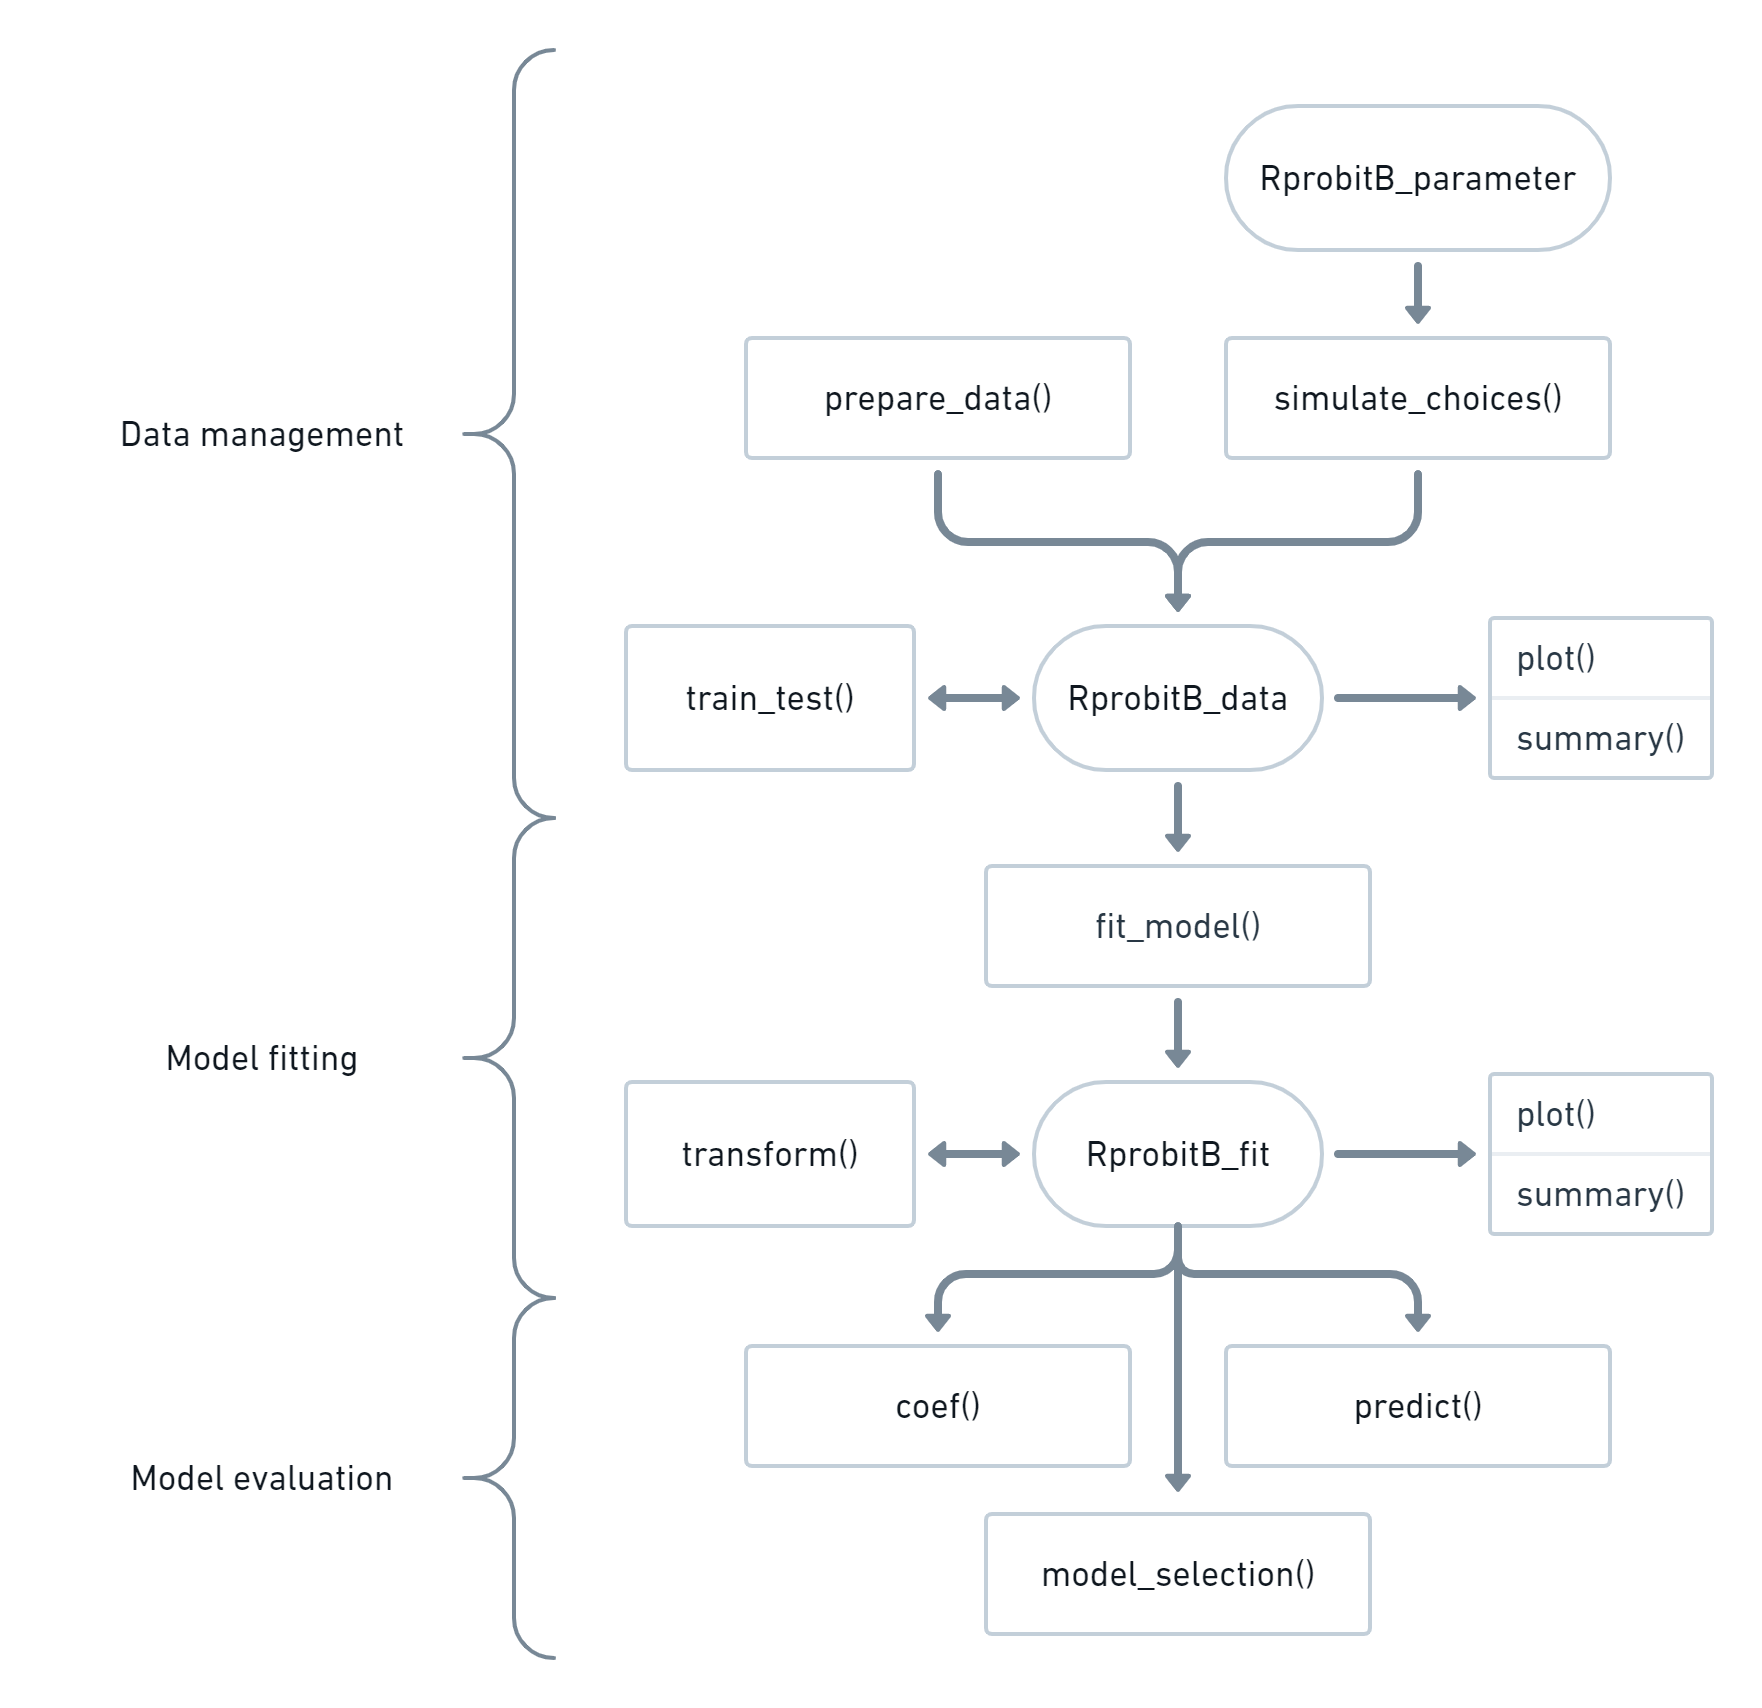
\includegraphics{flowchart.png}
  \caption{Flowchart of the main \pkg{RprobitB} functionalities (rectangles) and objects (ovals).}
  \label{fig:flowchart}
\end{figure}

\section{The probit model} \label{sec:probit_model}

This section briefly defines the probit model. For the model's data input, assume that we know the choices of $N$ deciders choosing between $J \geq 2$ alternatives at each of $T$ choice occasions.\footnote{The number $T$ of choice occasions is the same for each decider here for notational simplicity. However, \pkg{RprobitB} allows for unbalanced panels, i.e.\ varying $T$. Of course, the cross-sectional case $T = 1$ is possible.} Specific to each decider, alternative and choice occasion, we observe $P$ covariates, a linear combination of which explains the choices:
\begin{equation}
  \label{eq:utility}
  U_{ntj} = X_{ntj}'\beta_n + \epsilon_{ntj}
\end{equation}
for $n=1,\dots,N$, $t=1,\dots,T$ and $j=1,\dots,J$. Here, $X_{ntj}$ is a (column) vector of $P$ characteristics specific to alternative $j$ as faced by decider $n$ at choice occasion $t$, $\beta_n \in {\mathbb R}^{P}$ is the coefficient vector of $n$, and $(\epsilon_{nt:}) = (\epsilon_{nt1},\dots,\epsilon_{ntJ})' \sim \text{MVN}_{J} (0,\Sigma)$ is the model's error term vector for $n$ at $t$.

The value $U_{ntj}$ on the left-hand side of equation \eqref{eq:utility} can be interpreted as the decider's utility. It is unobserved by the researcher, but we assume that the deciders know their utilities for each alternative and make a choice which is consistent with utility maximization.\footnote{Utility maximizing behavior is a common assumption in econometric models. However, studies have shown that humans do not decide in this rational sense in general \citep{Hewig:2011}.} Therefore, we link
\begin{equation}
   \label{eq:link}
   y_{nt} = \operatorname*{argmax}_{j = 1,\dots,J} U_{ntj},
\end{equation}
where $y_{nt}=j$ denotes the event that decider $n$ chooses $j$ at $t$.

Equation \eqref{eq:utility} has a decider-specific coefficient vector $\beta_n$. Some entries of $\beta_n$ can be fixed across deciders, in which case the coefficient vector is of the form $(\alpha, \beta_n)$, where $\alpha$ are $P_f$ coefficients that are constant across deciders and $\beta_n$ are $P_r$ decider-specific coefficients, $P_f + P_r = P$. The decider-specific coefficients are assumed to be realizations of an underlying distribution, a so-called mixing distribution \citep[Ch.\ 6]{Train:2009}. This distribution characterizes heterogeneity among the deciders and allows for individual sensitivities as motivated in the introduction.

Choosing an appropriate mixing distribution is a notoriously difficult task of the model specification. In many applications, different types of standard parametric distributions (including the normal, log-normal, uniform and tent distribution) are tried in conjunction with a likelihood value-based model selection \citep[pp.\ 136 ff.\ ]{Train:2009}. Instead, \pkg{RprobitB} implements the approach of \cite{Oelschlaeger:2020} to approximate any underlying mixing distribution by a mixture of $P_r$-variate Gaussian densities $\phi_{P_r}$ with mean vectors $b=(b_c)_{c}$ and covariance matrices $\Omega=(\Omega_c)_{c}$ using $C$ components:
\begin{align*}
\beta_n\mid b,\Omega \sim \sum_{c=1}^{C} s_c \phi_{P_r} (\cdot \mid b_c,\Omega_c).
\end{align*}
Here, $(s_c)_{c}$ are weights satisfying $0 < s_c\leq 1$ for $c=1,\dots,C$ and $\sum_c s_c=1$. One interpretation of the latent class model is obtained by introducing variables $z=(z_n)_n$, allocating each decision maker $n$ to class $c$ with probability $s_c$, i.e.\
\begin{align*}
\text{Prob}(z_n=c)=s_c \land \beta_n \mid z,b,\Omega \sim \phi_{P_r}(\cdot \mid b_{z_n},\Omega_{z_n}).
\end{align*}
This interpretation allows for decider classifications, see Section \ref{subsec:dp_update} for an example.

Finally, the probit model requires normalization, because any utility model is invariant towards the level and the scale of utility \citep[Ch.\ 2]{Train:2009}. We therefore normalize the model by taking differences in \eqref{eq:utility} and fixing one error term variance:
\begin{equation}
\label{eq:utility_diff}
\tilde{U}_{ntj} = \tilde{X}_{ntj}' \beta + \tilde{\epsilon}_{ntj},
\end{equation}
where (choosing some alternative $k \in \{1,\dots,J\}$ as the reference), $\tilde{U}_{ntj} = U_{ntj} - U_{ntk}$, $\tilde{X}_{ntj} = X_{ntj} - X_{ntk}$, and $\tilde{\epsilon}_{ntj} = \epsilon_{ntj} - \epsilon_{ntk}$ for $j\neq k$. The error term differences $(\tilde{\epsilon}_{nt:}) = (\tilde{\epsilon}_{nt1},...,\tilde{\epsilon}_{nt(J-1)})'$ again are multivariate normally distributed with mean 0 but transformed covariance matrix $\tilde{\Sigma}$, in which one diagonal element is fixed to a positive number.\footnote{Fixing one element of $\tilde{\Sigma}$ determines the utility scale. Fixing one fixed effect (i.e.\ one entry of $\alpha$) serves the same purpose. Both alternatives are implemented in \pkg{RprobitB}, see Section \ref{subsec:estimation_routine}.}

\section{Choice data} \label{sec:choice_data}

\pkg{RprobitB} requests that choice data sets are (a) of class \class{data.frame}, (b) in wide format (that means each row provides the full information for one choice occasion), (c) contain a column with unique identifiers for each decision maker (and optionally each choice occasion), (d) contain a column with the observed choices (required for model fitting but not for prediction), and (e) contain columns for the values of (alternative and/or decider specific) covariates. The underlying set of choice alternatives is assumed to be mutually exclusive (one can choose one and only one alternative that are all different), exhaustive (the alternatives do not leave other options open), and finite \citep[Ch.\ 2]{Train:2009}. Alternatives can be considered as ordered (e.g.\ the level of agreement on a Likert-type rating scale, cf.\ Section \ref{subsec:ordered_alternatives}), and additionally full rankings of the alternatives can be provided (e.g.\ when asking the respondent to rank all available alternatives from best to worst, cf.\ Section \ref{subsec:ranked_choices}).

\subsection{Different types of covariates} \label{subsec:covariate_types}

Different covariate types can be considered: covariates that are constant across alternatives (e.g.\ a car buyer's income), covariates that are alternative specific (e.g.\ the car's price), covariates with a generic coefficient (e.g.\ paying the same amount of money for car company A versus B should make no difference), and covariates that have alternative specific coefficients (e.g.\ the range of an electric car might be of more importance than for other types of propulsion). To allow for these different types, we generalize equation \eqref{eq:utility} to
\begin{align}
  \label{eq:utility_gen}
  U_{ntj} = \beta_{0j} + A_{ntj} \beta_1 + B_{nt} \beta_{2j} + C_{ntj} \beta_{3j} + \epsilon_{ntj}.
\end{align}
Here, the covariates $A$ and $C$ depend on the alternative $j$, while $B$ is only decider and choice occasion specific. The coefficient $\beta_1$ for $A$ is generic (i.e.\ the same for each alternative), whereas $\beta_{2j}$ and $\beta_{3j}$ for $B$ and $C$ are alternative specific. The intercept $\beta_0j$ is called alternative specific constant (ASC). ASCs capture the average effect on the alternative's utility of all factors that are not included in the model.

Note that the full collections $(\beta_{0j})_{j=1,\dots,J}$ of ASCs and $(\beta_{2j})_{j=1,\dots,J}$ of coefficients for covariate type $B$ are not identified. This is because we took utility differences for model normalization (cf.\ Section \ref{sec:probit_model}), and hence one coefficient is a linear combination of the others, respectively. We therefore fix $\beta_{0k}$ and $\beta_{2k}$ to 0 for one base alternative $k$. The coefficients $(\beta_{0j})_{j\neq k}$ and $(\beta_{2j})_{j\neq k}$ then have to be interpreted with respect to $k$.

\subsection{Formula framework} \label{subsec:formula}

Specifying equation \eqref{eq:utility_gen} in \proglang{R} requires a flexible formula framework. \pkg{RprobitB} can interpret a \class{formula} object of the form \code{choice ~ A | B | C}, where \code{choice} is the name of the dependent variable (the discrete choice we aim to explain), and \code{A}, \code{B}, and \code{C} are the different covariate types of Section \ref{subsec:covariate_types}.\footnote{This formula framework is adapted from \pkg{mlogit}.}

The framework has the following rules. ASCs are added to the model per default. They can be removed by adding \code{+ 0} in the second spot, e.g.\ \code{choice ~ A | B + 0 | C}. To exclude covariates of the backmost categories, use either \code{0}, e.g.\ \code{choice ~ A | B | 0} or just leave this part out and write \code{choice ~ A | B}. However, to exclude covariates of front categories, we have to use \code{0}, e.g.\ \code{choice ~ 0 | B}. To include more than one covariate of the same category, use \code{+}, e.g.\ \code{choice ~ A1 + A2 | B}. If we don't want to include any covariates of the second category but want to estimate ASCs, add \code{1} in the second spot, e.g.\ \code{choice ~ A | 1 | C}. The expression \code{choice ~ A | 0 | C} is interpreted as no covariates of the second category and no alternative specific constants.

\subsection{Preparing data for estimation} \label{subsec:prepare_data}

Before model estimation, any choice data set \code{choice\_data} must pass the \fct{prepare\_data} function together with a formula object \code{form} introduced in Section \ref{subsec:formula}:

\begin{Schunk}
\begin{Sinput}
> data <- prepare_data(form = form, choice_data = choice_data)
\end{Sinput}
\end{Schunk}

The function performs compatibility checks and data transformations, and returns an object of class \class{RprobitB\_data} that can be fed into the estimation routine \fct{fit\_model} (that we introduce in Section \ref{sec:model_fitting}). The following arguments of \fct{prepare\_data} are optional:
\begin{itemize}
  \item \code{re}: A character vector of covariate names in \code{form} with random effects. Per default \code{re = NULL}, i.e.\ no random effects.
  \item \code{alternatives}: A character vector of the alternative names, defining the choice set. If not specified, all alternatives chosen in \code{choice\_data} are considered.
  \item \code{ordered} and \code{ranked}: Two booleans, that are set to \code{FALSE} per default. If set to \code{TRUE}, the alternatives are interpreted as ordered, or the choices are interpreted as ranked, respectively. See Sections \ref{subsec:ordered_alternatives} and \ref{subsec:ranked_choices} for details.
  \item \code{base}: One element of \code{alternatives} specifying the base alternative (cf.\ Section \ref{subsec:covariate_types}). Per default, \code{base} is the last element of \code{alternatives}.
  \item \code{id} and \code{idc}: The names of the columns in \code{choice_data} that contain unique identifier for each decision maker and for each choice occasion, respectively. Per default, \code{id = "id"} and \code{idc = NULL}, in which case the choice occasion identifier are generated by the appearance of the choices in the \code{choice\_data}.
  \item \code{standardize}: A character vector of variable names of \code{form} that get standardized, i.e.\ rescaled to have a mean of 0 and a standard deviation of 1 (none per default).
  \item \code{impute}: A character, specifying how to handle missing covariates in \code{choice\_data}. Options are \code{"complete\_cases"} (removing rows that contain missing entries, which is the default behavior), \code{"zero"} (replacing missing entries by 0), and \code{"mean"} (imputing missing entries by the covariate mean).
\end{itemize}

\paragraph{Example 1: Train trips.}

The \pkg{mlogit} package contains the data set \code{Train} with 2929 stated choices of 235 deciders between two fictional train trip alternatives \code{A} and \code{B}. The trip alternatives are characterized by their \code{price}, the travel \code{time}, the level of \code{comfort} (the lower the value the higher the comfort), and the number of \code{change}s. The data is in wide format; the columns \code{id} and \code{choiceid} identify the deciders and the choice occasions, respectively; the column \code{choice} provides the choices. For convenience, we transform \code{time} from minutes to hours and \code{price} from guilders to euros:

\begin{Schunk}
\begin{Sinput}
> data("Train", package = "mlogit")
> Train$price_A <- Train$price_A / 100 * 2.20371
> Train$price_B <- Train$price_B / 100 * 2.20371
> Train$time_A <- Train$time_A / 60
> Train$time_B <- Train$time_B / 60
> str(Train)
\end{Sinput}
\begin{Soutput}
'data.frame':	2929 obs. of  11 variables:
 $ id       : int  1 1 1 1 1 1 1 1 1 1 ...
 $ choiceid : int  1 2 3 4 5 6 7 8 9 10 ...
 $ choice   : Factor w/ 2 levels "A","B": 1 1 1 2 2 2 2 2 1 1 ...
 $ price_A  : num  52.9 52.9 52.9 88.1 52.9 ...
 $ time_A   : num  2.5 2.5 1.92 2.17 2.5 ...
 $ change_A : num  0 0 0 0 0 0 0 0 0 0 ...
 $ comfort_A: num  1 1 1 1 1 0 1 1 0 1 ...
 $ price_B  : num  88.1 70.5 88.1 70.5 70.5 ...
 $ time_B   : num  2.5 2.17 1.92 2.5 2.5 ...
 $ change_B : num  0 0 0 0 0 0 0 0 0 0 ...
 $ comfort_B: num  1 1 0 0 0 0 1 0 1 0 ...
\end{Soutput}
\end{Schunk}

For demonstration, we include all choice characteristics into our probit model, connect them to generic and fixed coefficients, and exclude ASCs:

\begin{Schunk}
\begin{Sinput}
> form <- choice ~ price + time + comfort + change | 0
\end{Sinput}
\end{Schunk}

Passing \code{form} to \fct{prepare\_data} returns an \class{RprobitB\_data} object (which we fed into the estimation routine \fct{fit\_model} in Section \ref{sec:model_fitting}):

\begin{Schunk}
\begin{Sinput}
> data_train <- prepare_data(
+    form = form, choice_data = Train, id = "id", idc = "choiceid"
+  )
\end{Sinput}
\end{Schunk}

The data object can be inspected via its \fct{summary} and \fct{plot} methods:

\begin{Schunk}
\begin{Sinput}
> summary(data_train)
\end{Sinput}
\begin{Soutput}
                 count
deciders           235
choice occasions  5-19
total choices     2929
alternatives         2
- 'A'             1474
- 'B'             1455
\end{Soutput}
\end{Schunk}

\begin{Schunk}
\begin{Sinput}
> plot(data_train)
\end{Sinput}
\end{Schunk}
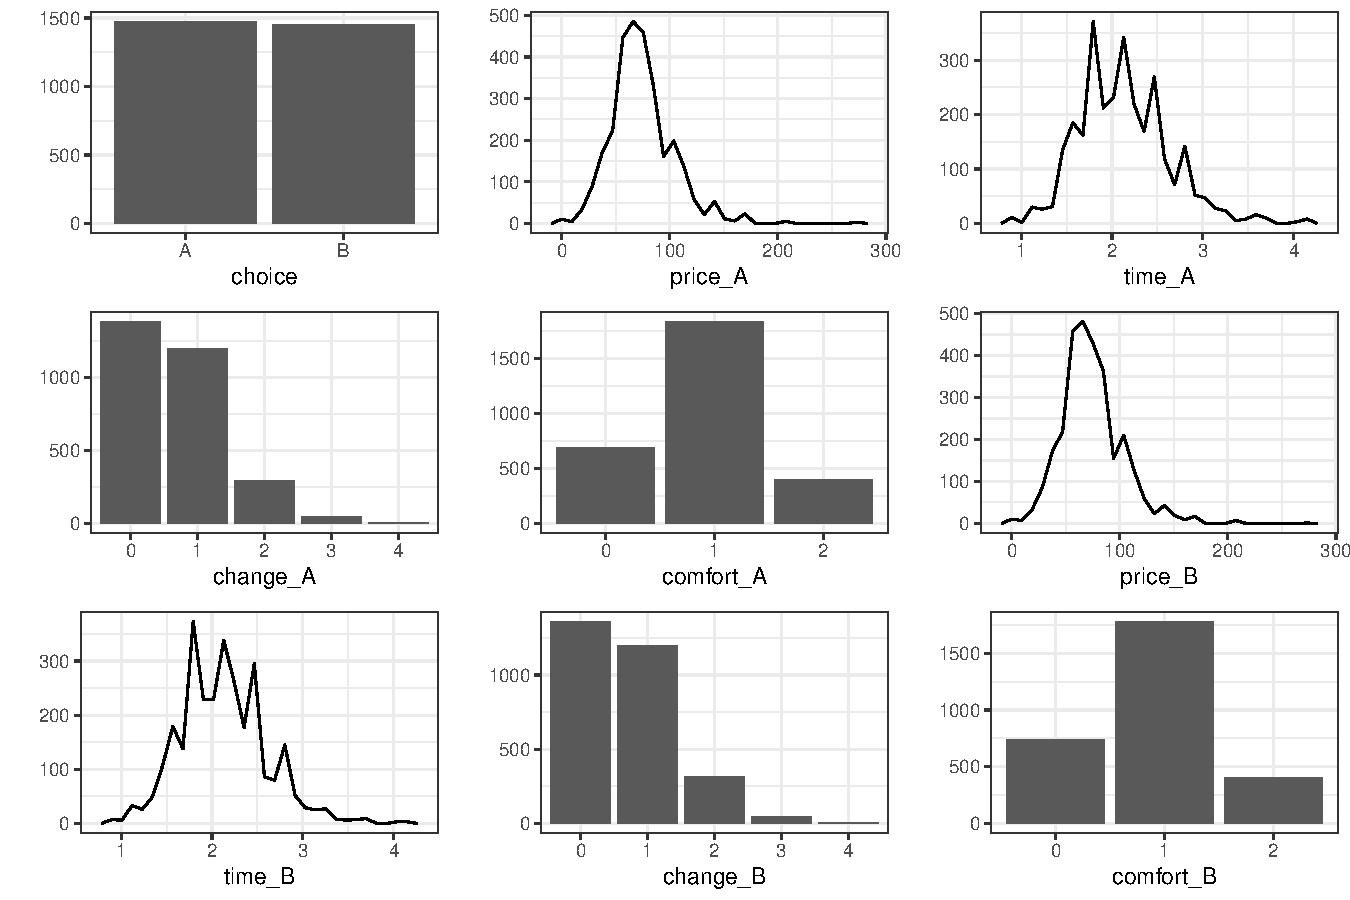
\includegraphics{rprobitb_oelschlaeger_bauer-train-data}

\subsection{Ordered alternatives} \label{subsec:ordered_alternatives}

The two choice alternatives in Example 1 are unordered. If we had asked "rate your train trip from 1 (horrible) to 7 (great)", then the respondents would choose their answer from a set of ordered alternatives. Ordered alternatives can by analyzed in \pkg{RprobitB} by setting \code{ordered = TRUE} in \fct{prepare\_data}. In this case, \code{alternatives} becomes a mandatory argument, with the alternative names ordered from worst to best.

In the ordered case, the concept of decider's having separate utilities for each alternative is no longer natural \citep[Ch.\ 7.4]{Train:2009}. Instead, we model only a single utility value
\begin{align*}
  U_{nt} = X_{nt}'\beta_n + \epsilon_{nt}
\end{align*}
per decider $n$ and choice occasion $t$, which we interpret as the "level of association" that $n$ has with the choice question. The utility value falls into discrete categories, which in turn are linked to the ordered alternatives $j=1,\dots,J$. Formally, the link in equation \eqref{eq:link} gets replaced by
\begin{align*}
   y_{nt} = \sum_{j = 1,\dots,J} j \cdot I(\gamma_{j-1} < U_{nt} \leq \gamma_{j}),
\end{align*}
with end points $\gamma_0 = -\infty$ and $\gamma_J = +\infty$, and thresholds $(\gamma_j)_{j=1,\dots,J-1}$. To ensure monotonicity of the thresholds, we rather estimate logarithmic threshold increments $d_j$ with $\gamma_j = \sum_{i=1,\dots,j} \exp{d_i}$, $j=1,\dots,J-1$.

Normalizing the ordered probit model with respect to the utility level differs from the unordered case: since we model only one utility value, we can no longer take utility differences, but instead fix $\gamma_1 = 0$. For scale normalization however, we again can either fix the variance of the (now univariate) normal distribution of the error term $\epsilon_{nt}$, or fix a fixed effect. Both options are available in \pkg{RprobitB} through the \code{scale} argument for the estimation routine \fct{fit\_model} (cf.\ Section \ref{subsec:estimation_routine}).\footnote{Note that there is even a third option for scale normalization: restricting the value space for the thresholds to a bounded interval also serves the purpose, but is not implemented.}

\subsection{Ranked choices} \label{subsec:ranked_choices}

Ranked choices are yet another variation: rather than recording only the single most preferred alternative, some surveys ask for a full ranking (from most preferred to least preferred) of all the alternatives, which reveals far more about the underlying preferences. Ranked choices can by analyzed in \pkg{RprobitB} by setting \code{ranked = TRUE} in \fct{prepare\_data}. In this case, the column of choices in \code{choice_data} must be of \class{character} type, containing for each choice occasion the full ranking of the available alternatives separated by commas, cf. Example 2. The ranked probit model follows directly from the basic multivariate model by replacing the differencing of equation \eqref{eq:utility_diff} such that the resulting utility vector is always negative, see \citep[Ch.\ 7.3]{Train:2009} for details.

\subsection{Simulating choice data} \label{subsec:simulate_choice_data}

The \fct{simulate\_choices} function simulates choice data from a pre-specified probit model. In order to simulate the choices of \code{N} deciders in \code{T} choice occasions\footnote{\code{T} can be either a positive number, representing a fixed number of choice occasions for each decision maker, or a vector of length \code{N} with decision maker specific numbers of choice occasions} among \code{J} alternatives,

\begin{Schunk}
\begin{Sinput}
> data <- simulate_choices(form = form, N = N, T = T, J = J)
\end{Sinput}
\end{Schunk}

where \code{form} is a model formula introduced in Section \ref{subsec:formula}. The function \fct{simulate\_choices} has the following optional arguments:
\begin{itemize}
  \item \code{re}, \code{ordered}, \code{ranked}, \code{base}, \code{standardize}: Analogue to \fct{prepare\_data} (cf.\ Section \ref{subsec:prepare_data}).
  \item \code{alternatives}: A character vector of length \code{J} with the names of the choice alternatives (per default the first \code{J} upper-case letters of the Roman alphabet).
  \item \code{covariates}: A named list of covariate values. Each element must be a vector of length equal to the number of choice occasions and named according to a covariate. Unspecified covariates are drawn from a standard normal distribution.
  \item \code{seed}: Optionally set a seed for the simulation.
\end{itemize}

The true model parameters are set at random per default. Alternatively, they can be specified via a named list for the function's \code{true\_parameter} argument. The list can contain contains
\begin{itemize}
  \item a numeric vector \code{alpha} with the fixed effects,
  \item the number \code{C} of latent classes (\code{C = 1} per default),
  \item a numeric vector \code{s} of length \code{C} with the class weights,
  \item a matrix \code{b} with the class means as columns,
  \item a matrix \code{Omega} with the class covariance matrices as columns,
  \item a matrix \code{Sigma\_full} (\code{Sigma}), the (differenced) error term covariance matrix,
  \item a matrix \code{beta} with the decision-maker specific coefficient vectors as columns,
  \item a numeric vector \code{z} of length \code{N} with elements in \code{1:C}, representing the class allocations,
  \item a numeric vector \code{d} of the logarithmic threshold increments in the ordered probit case.
\end{itemize}

\paragraph{Example 2: Simulated ranked choices.}
% Change to ranked
For illustration, we simulate the choices of \code{N = 100} deciders at \code{T = 30} choice occasions between the fictitious alternatives \code{alt1} and \code{alt2}. The choices are explained by the alternative specific covariates \code{var1} and \code{var3}. Covariate \code{var2} is only choice occasion specific but connected to a random effect, as well as the ASCs:

\begin{Schunk}
\begin{Sinput}
> N <- 100
> T <- 30
> alternatives <- c("alt1", "alt2")
> form <- choice ~ var1 | var2 | var3
> re <- c("ASC","var2")
\end{Sinput}
\end{Schunk}

The \fct{overview\_effects} function provides an overview of the effect types:

\begin{Schunk}
\begin{Sinput}
> overview_effects(form = form, re = re, alternatives = alternatives)
\end{Sinput}
\begin{Soutput}
     effect as_value as_coef random
1      var1     TRUE   FALSE  FALSE
2 var3_alt1     TRUE    TRUE  FALSE
3 var3_alt2     TRUE    TRUE  FALSE
4 var2_alt1    FALSE    TRUE   TRUE
5  ASC_alt1    FALSE    TRUE   TRUE
\end{Soutput}
\end{Schunk}

The model has three fixed effects (\code{random = FALSE}), consequently the vector \code{alpha} must be of length 3, where the elements 1 to 3 correspond to \code{var1}, \code{var3\_alt1}, and \code{var3\_alt2}, respectively. Additionally, the model has two random effects (\code{random = TRUE}), hence the matrix \code{b} must be of dimension \code{2 x C}, where row 1 and 2 correspond to \code{var2\_alt1} and \code{ASC\_alt1}, respectively. We specify \code{C = 2} latent classes in the data generating process, which we will reproduce in Sections \ref{subsec:latent_classes} and \ref{subsec:weight_update}.

As simulation parameters, we specify $\alpha = \begin{pmatrix} -1 & 0 & 1 \end{pmatrix}^t$, class weights $s = \begin{pmatrix} 0.7 & 0.3 \end{pmatrix}$, class means $b_1 = \begin{pmatrix} 2 & -0.5 \end{pmatrix}^t$ and $b_2 = \begin{pmatrix} 1 & 1 \end{pmatrix}^t$, and $\Sigma = 1$. The class covariances $\Omega_1$ and $\Omega_2$ remain unspecified and hence are set at random.

\begin{Schunk}
\begin{Sinput}
> data_sim <- simulate_choices(
+    form = form, N = N, T = T, J = 2,
+    re = re, alternatives = alternatives, seed = 1,
+    true_parameter = list(
+      alpha = c(-1,0,1), C = 2, s = c(0.7,0.3),
+      b = matrix(c(2,-0.5,1,1), ncol = 2), Sigma = 1)
+  )
\end{Sinput}
\end{Schunk}

The \fct{plot} method of \class{RprobitB\_data} objects has the optional argument \code{by\_choice}. Setting \code{by\_choice = TRUE} visualizes the (randomly drawn) covariates grouped by the chosen alternatives:

\begin{Schunk}
\begin{Sinput}
> plot(data_sim, by_choice = TRUE)
\end{Sinput}
\end{Schunk}
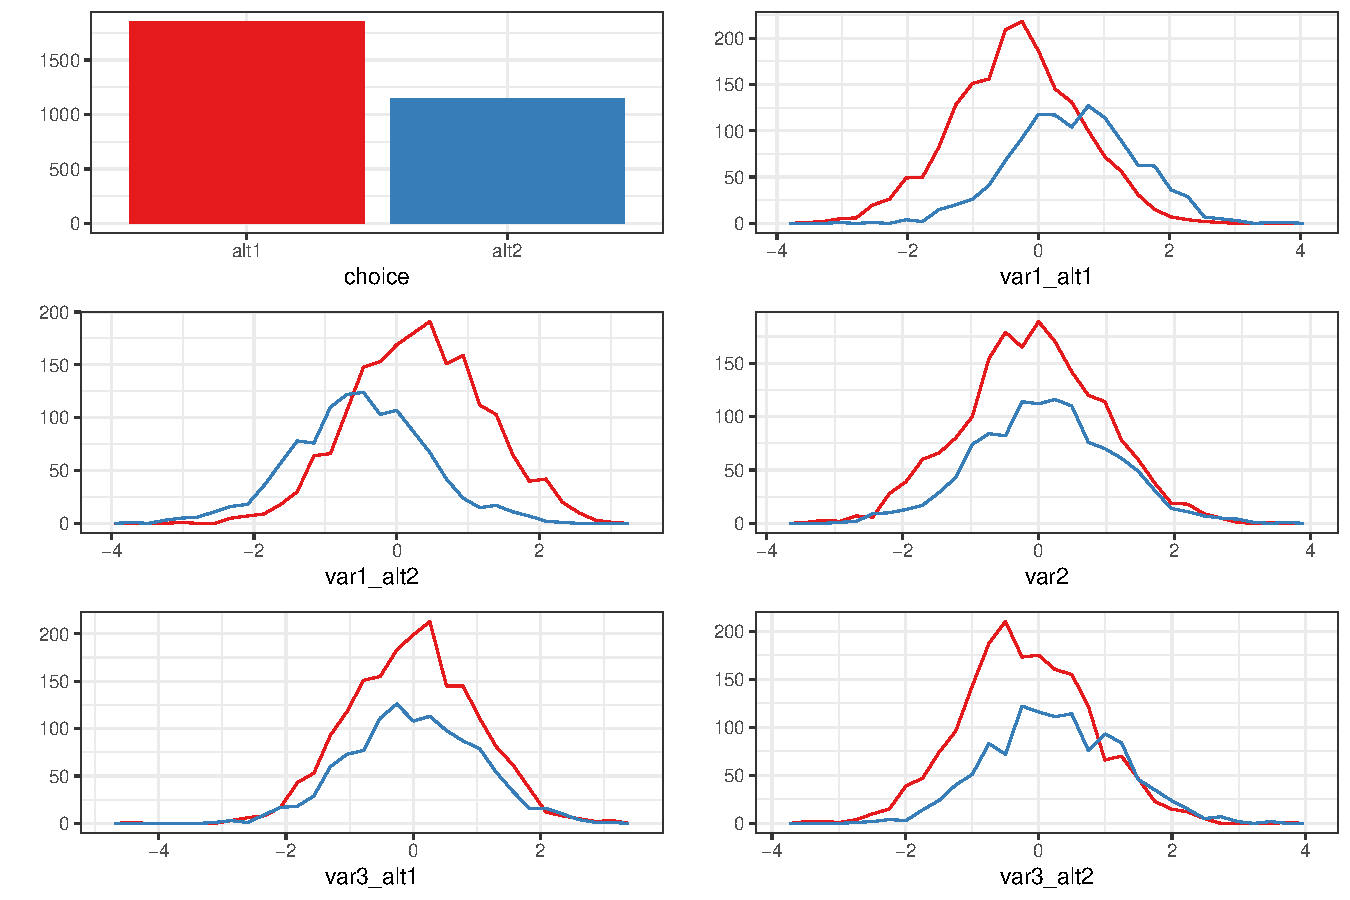
\includegraphics{rprobitb_oelschlaeger_bauer-sim-data}

The graphic is consistent with our model specification: for example, covariate \code{var1} was specified to have a negative effect on \code{alt1}, because the coefficient of \code{var1} (the first value of \code{alpha}) is negative $(-1)$. Hence, higher values of \code{var1\_alt1} correspond more frequently to choice \code{alt2} (upper-right panel).

\section{Model fitting} \label{sec:model_fitting}

\pkg{RprobitB} estimates the probit model in a Bayesian framework that builds upon the work of \cite{McCulloch:1994}, \cite{Nobile:1998}, \cite{Allenby:1998}, and \cite{Imai:2005}. A key ingredient is the concept of data augmentation \citep{Albert:1993}, which treats the latent utilities in model equation \eqref{eq:utility} as additional parameters. Then, conditional on these parameters, the probit model constitutes a standard Bayesian linear regression set-up. Its posterior distribution can be approximated via Gibbs sampling.

In the following, we list the prior distributions for the model parameters, formulate the conditional posterior distributions, introduce the estimation routine \fct{fit\_model}, and apply it to the two examples from the previous section. The remainder of this section is devoted to the estimation of latent class models and the implemented class updating schemes.

\subsection{Prior and posterior distributions} \label{subsec:prior_and_posterior}

We a priori assume the following (conjugate) parameter distributions:
\begin{itemize}
  \item $(s_1,\dots,s_C)\sim D_C(\delta)$, where $D_C(\delta)$ denotes the $C$-dimensional Dirichlet distribution with concentration parameter vector $\delta = (\delta_1,\dots,\delta_C)$,
  \item $\alpha\sim \text{MVN}_{P_f}(\psi,\Psi)$, where $\text{MVN}_{P_f}$ denotes the $P_f$-dimensional normal distribution with mean $\psi$ and covariance $\Psi$,
  \item $b_c \sim \text{MVN}_{P_r}(\xi,\Xi)$, independent for all $c$,
  \item $\Omega_c \sim W^{-1}_{P_r}(\nu,\Theta)$, independent for all $c$, where $W^{-1}_{P_r}(\nu,\Theta)$ denotes the $P_r$-dimensional inverse Wishart distribution with $\nu$ degrees of freedom and scale matrix $\Theta$,
  \item $\tilde{\Sigma} \sim W^{-1}_{J-1}(\kappa,\Lambda)$,
  \item and $\gamma \sim MVN_{J-2}(\zeta,Z)$.
\end{itemize}

These priors imply the following conditional posterior distributions (we are closely following \cite{Oelschlaeger:2020}):
\begin{itemize}
  \item The class weights are drawn from the Dirichlet distribution
  \begin{align*}
  (s_1,\dots,s_C)\mid \delta,z \sim D_C(\delta_1+m_1,\dots,\delta_C+m_C),
  \end{align*}
  where $m_c=\#\{n:z_n=c\}$ denotes the current absolute size of class $c$. The model is invariant to permutations of the class labels $1,\dots,C$. We therefore accept an update only if the ordering $s_1>\dots>s_C$ still holds (thereby ensuring a unique class labeling).
  \item The allocation variables $(z_n)_n$ are updated independently for all $n$ via
  \begin{align*}
  \text{Prob}(z_n=c\mid s,\beta,b,\Omega )=\frac{s_c\phi_{P_r}(\beta_n\mid b_c,\Omega_c)}{\sum_c s_c\phi_{P_r}(\beta_n\mid b_c,\Omega_c)}.
  \end{align*}
  \item The class means $(b_c)_c$ are updated independently for all $c$ via
  \begin{align*}
  b_c\mid \Xi,\Omega,\xi,z,\beta \sim\text{MVN}_{P_r}\left( \mu_{b_c}, \Sigma_{b_c}  \right),
  \end{align*}
  $\mu_{b_c}=(\Xi^{-1}+m_c\Omega_c^{-1})^{-1}(\Xi^{-1}\xi +m_c\Omega_c^{-1}\bar{b}_c)$, $\Sigma_{b_c}=(\Xi^{-1}+m_c\Omega_c^{-1})^{-1}$, $\bar{b}_c=m_c^{-1}\sum_{n:z_n=c} \beta_n$.
    \item The class covariance matrices $(\Omega_c)_c$ are updated independently for all $c$ via
  \begin{align*}
  \Omega_c \mid \nu,\Theta,z,\beta,b \sim W^{-1}_{P_r}(\mu_{\Omega_c},\Sigma_{\Omega_c}),
  \end{align*}
  $\mu_{\Omega_c}=\nu+m_c$, $\Sigma_{\Omega_c}=\Theta^{-1} + \sum_{n:z_n=c} (\beta_n-b_c)(\beta_n-b_c)'$.
  \item Independently for all $n,t$ and conditionally on the other components, the differenced utility vectors $(\tilde{U}_{nt:})$ follow a $(J-1)$-variate truncated normal distribution, where the truncation points are determined by the choices $y_{nt}$. To sample from a truncated multivariate normal distribution, we apply a sub-Gibbs sampler (analogue to \cite{Geweke:1998}):
  \begin{align*}
  \tilde{U}_{ntj} \mid \tilde{U}_{nt(-j)},y_{nt},\tilde{\Sigma},\tilde{W},\alpha,\tilde{X},\beta
  \sim \mathcal{N}(\mu_{\tilde{U}_{ntj}},\Sigma_{\tilde{U}_{ntj}}) \cdot \begin{cases}
  1(\tilde{U}_{ntj}>\max(\tilde{U}_{nt(-j)},0) ) & \text{if}~ y_{nt}=j\\
  1(\tilde{U}_{ntj}<\max(\tilde{U}_{nt(-j)},0) ) & \text{if}~ y_{nt}\neq j
  \end{cases},
  \end{align*}
  where $\tilde{U}_{nt(-j)}$ denotes the vector $(\tilde{U}_{nt:})$ without the element $\tilde{U}_{ntj}$, $\mathcal{N}$ the univariate normal distribution, $\Sigma_{\tilde{U}_{ntj}} = 1/(\tilde{\Sigma}^{-1})_{jj}$, and
  \begin{align*}
  \mu_{\tilde{U}_{ntj}} = \tilde{W}_{ntj}'\alpha + \tilde{X}_{ntj}'\beta_n - \Sigma_{\tilde{U}_{ntj}} (\tilde{\Sigma}^{-1})_{j(-j)}   (\tilde{U}_{nt(-j)} - \tilde{W}_{nt(-j)}'\alpha - \tilde{X}_{nt(-j)}' \beta_n ),
  \end{align*}
  where $(\tilde{\Sigma}^{-1})_{jj}$ denotes the $(j,j)$-th element of $\tilde{\Sigma}^{-1}$, $(\tilde{\Sigma}^{-1})_{j(-j)}$ the $j$-th row without the $j$-th entry, $\tilde{W}_{nt(-j)}$ and $\tilde{X}_{nt(-j)}$ the differenced covariate matrices connected to fixed and random effects, respectively, with the $j$-th column removed.

  In the ranked case ...

  In the ordered case ...
  \item Updating the fixed coefficient vector $\alpha$ is achieved by applying the formula for Bayesian linear regression of the regressors $\tilde{W}_{nt}$ on the regressands $(\tilde{U}_{nt:})-\tilde{X}_{nt}'\beta_n$, i.e.\
  \begin{align*}
  \alpha \mid \Psi,\psi,\tilde{W},\tilde{\Sigma},\tilde{U},\tilde{X},\beta \sim \text{MVN}_{P_f}(\mu_\alpha,\Sigma_\alpha),
  \end{align*}
  $\mu_\alpha = \Sigma_\alpha (\Psi^{-1}\psi + \sum_{n=1,t=1}^{N,T} \tilde{W}_{nt} \tilde{\Sigma}^{-1} ((\tilde{U}_{nt:})-\tilde{X}_{nt}'\beta_n) )$, $\Sigma_\alpha = (\Psi^{-1} + \sum_{n=1,t=1}^{N,T} \tilde{W}_{nt}\tilde{\Sigma}^{-1} \tilde{W}_{nt}^{'} )^{-1}$.
  \item Analogously to $\alpha$, the random coefficients $(\beta_n)_n$ are updated independently via
  \begin{align*}
  \beta_n \mid \Omega,b,\tilde{X},\tilde{\Sigma},\tilde{U},\tilde{W},\alpha \sim \text{MVN}_{P_r}(\mu_{\beta_n},\Sigma_{\beta_n}),
  \end{align*}
  $\mu_{\beta_n} = \Sigma_{\beta_n} (\Omega_{z_n}^{-1}b_{z_n} + \sum_{t=1}^{T} \tilde{X}_{nt} \tilde{\Sigma}^{-1} (\tilde{U}_{nt}-\tilde{W}_{nt}'\alpha) )$, $\Sigma_{\beta_n} = (\Omega_{z_n}^{-1} + \sum_{t=1}^{T} \tilde{X}_{nt}\tilde{\Sigma}^{-1} \tilde{X_{nt}}^{'} )^{-1}$.
    \item The covariance matrix $\tilde{\Sigma}$ of the error term differences is updated by means of
  \begin{align*}
  \tilde{\Sigma} \mid \kappa,\Lambda,\tilde{U},\tilde{W},\alpha,\tilde{X},\beta \sim W^{-1}_{J-1}(\kappa+NT,\Lambda+S),
  \end{align*}
  where $S = \sum_{n=1,t=1}^{N,T} \tilde{\varepsilon}_{nt} \tilde{\varepsilon}_{nt}'$ and $\tilde{\varepsilon}_{nt} = (\tilde{U}_{nt:}) - \tilde{W}_{nt}'\alpha - \tilde{X}_{nt}'\beta_n$.
\end{itemize}

The Gibbs samples obtained from this updating scheme (except for $s$ and $z$ draws) lack identification with respect to the scale (cf.\ Section \ref{sec:probit_model}). Subsequent to the sampling and for the $i$-th updates in each iteration $i$, we therefore apply the normalization $\alpha^{(i)} \cdot \omega^{(i)}$, $b_c^{(i)} \cdot \omega^{(i)}$, $\tilde{U}_{nt}^{(i)} \cdot \omega^{(i)}$, $\beta_n^{(i)} \cdot \omega^{(i)}$, $\Omega_c^{(i)} \cdot (\omega^{(i)})^2$, and $\tilde{\Sigma}^{(i)} \cdot (\omega^{(i)})^2$, where either $\omega^{(i)} = \sqrt{\text{const} / (\tilde{\Sigma}^{(i)})_{jj}}$ with $(\tilde{\Sigma}^{(i)})_{jj}$ the $j$-th diagonal element of $\tilde{\Sigma}^{(i)}$, $1\leq j \leq J-1$, or alternatively $\omega^{(i)} = \text{const} / \alpha^{(i)}_p$ for some coordinate $1\leq p \leq P_f$ of the $i$-th draw for the coefficient vector $\alpha$. Here, $\text{const}$ is a constant to specify custom utility scales.

\subsection{The estimation routine} \label{subsec:estimation_routine}

The Gibbs sampling scheme can be executed via the function call

\begin{Schunk}
\begin{Sinput}
> fit_model(data = data)
\end{Sinput}
\end{Schunk}

where \code{data} is an \class{RprobitB\_data} object (cf.\ Section \ref{sec:choice_data}). Optional arguments are:

\begin{itemize}
  \item \code{scale}: A character which determines the utility scale (cf.\ Section \ref{sec:probit_model}). It is of the form \code{"<parameter> := <value>"}, where \code{<parameter>} is either the name of a fixed effect or \code{Sigma\_<j>} for the \code{<j>}-th diagonal element of \code{Sigma}, and \code{<value>} is the value of the fixed parameter (i.e.\ $\text{const}$ introduced in Section \ref{subsec:prior_and_posterior}). Per default \code{scale = "Sigma\_1 := 1"}, i.e.\ the first error-term variance is fixed to 1.
  \item \code{R}: The number of iterations of the Gibbs sampler. The default is \code{R = 1000}.
  \item \code{B}: The length of the burn-in period (\code{B = R/2} per default).\footnote{The theory behind Gibbs sampling constitutes that the sequence of samples produced by the
updating scheme is a Markov chain with stationary distribution equal to the desired joint posterior distribution. It takes a certain number of iterations for that stationary distribution to be approximated reasonably well. Therefore, it is common practice to discard the first \code{B} out of \code{R} samples (the so-called burn-in period).}
  \item \code{Q}: The thinning factor for the Gibbs samples (\code{Q = 1} per default).
  \item \code{print\_progress}: A boolean, determining whether to print the Gibbs sampler progress.
  \item \code{prior}: A named list of parameters for the prior distributions. Default values are documented in the \fct{check\_prior} function, see \code{help(check\_prior, package = "RprobitB")}.
\end{itemize}

\paragraph{Example 1: Train trips (cont.).}

Recall the \code{Train} data set of stated train trip alternatives, characterized by their \code{price}, \code{time}, number of \code{change}s, and level of \code{comfort}. From this data, we previously build the \class{RprobitB\_data} object \code{data\_train}, which we now pass to the estimation routine \fct{fit\_model}. For model normalization, we fix the \code{price} coefficient to \code{-1}, which has the advantage that we can interpret the other coefficients as monetary values:

\begin{Schunk}
\begin{Sinput}
> model_train <- fit_model(data = data_train, R = 1000, scale = "price := -1")
\end{Sinput}
\end{Schunk}

The estimated coefficients (using the mean of the Gibbs samples as a point estimate) can be visualized via

\begin{Schunk}
\begin{Sinput}
> plot(coef(model_train), sd = 3)
\end{Sinput}
\end{Schunk}
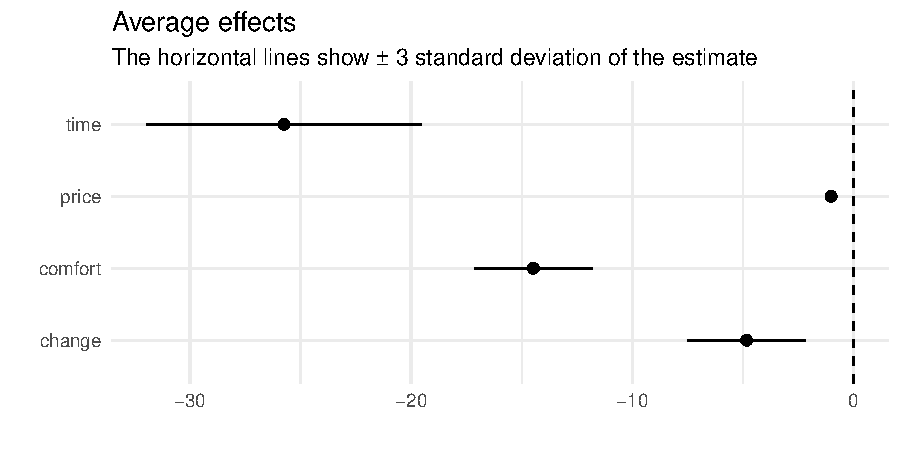
\includegraphics{rprobitb_oelschlaeger_bauer-coef-model-train}

The results indicate that the deciders value one hour travel time by about 26 euros, an additional change by 5 euros, and a more comfortable class by 15 euros.\footnote{We note that these results are consistent with the ones that are presented in a vignette of \pkg{mlogit} entitled "The random parameters (or mixed) logit model" on the same data set but using the logit model.} Calling the \fct{summary} method on the estimated \class{RprobitB\_fit} object yields additional information about the (transformed) Gibbs samples. The method receives a list \code{FUN} of arbitrary functions that can compute point estimates of the Gibbs samples, per default \fct{mean} for the arithmetic mean, \fct{stats::sd} for the standard deviation, and \fct{R\_hat} for the Gelman-Rubin statistic \citep{Gelman:1992}\footnote{A Gelman-Rubin statistic (a lot) greater than 1 indicates convergence issues of the Gibbs sampler.}:

\begin{Schunk}
\begin{Sinput}
> FUN <- c("mean" = mean, "sd" = stats::sd, "R^" = RprobitB::R_hat)
> summary(model_train, FUN = FUN)
\end{Sinput}
\begin{Soutput}
Probit model
Formula: choice ~ price + time + comfort + change | 0 
R: 1000, B: 500, Q: 1

Utility normalization
Level: Utility differences with respect to alternative 'B'.
Scale: Coefficient of effect 'price' (alpha_1) fixed to -1.

Gibbs sample statistics
          mean      sd      R^
 alpha
                              
     1   -1.00    0.00    1.00
     2  -25.95    2.08    1.00
     3  -14.52    0.84    1.00
     4   -4.96    0.87    1.03

 Sigma
                              
   1,1  660.03   58.54    1.00
\end{Soutput}
\end{Schunk}

Calling the \fct{plot} method with the additional argument \code{type = "trace"} plots the trace of the transformed and thinned Gibbs samples after the burn-in:

\begin{Schunk}
\begin{Sinput}
> par(mfrow = c(1,2))
> plot(model_train, type = "trace")
\end{Sinput}
\end{Schunk}
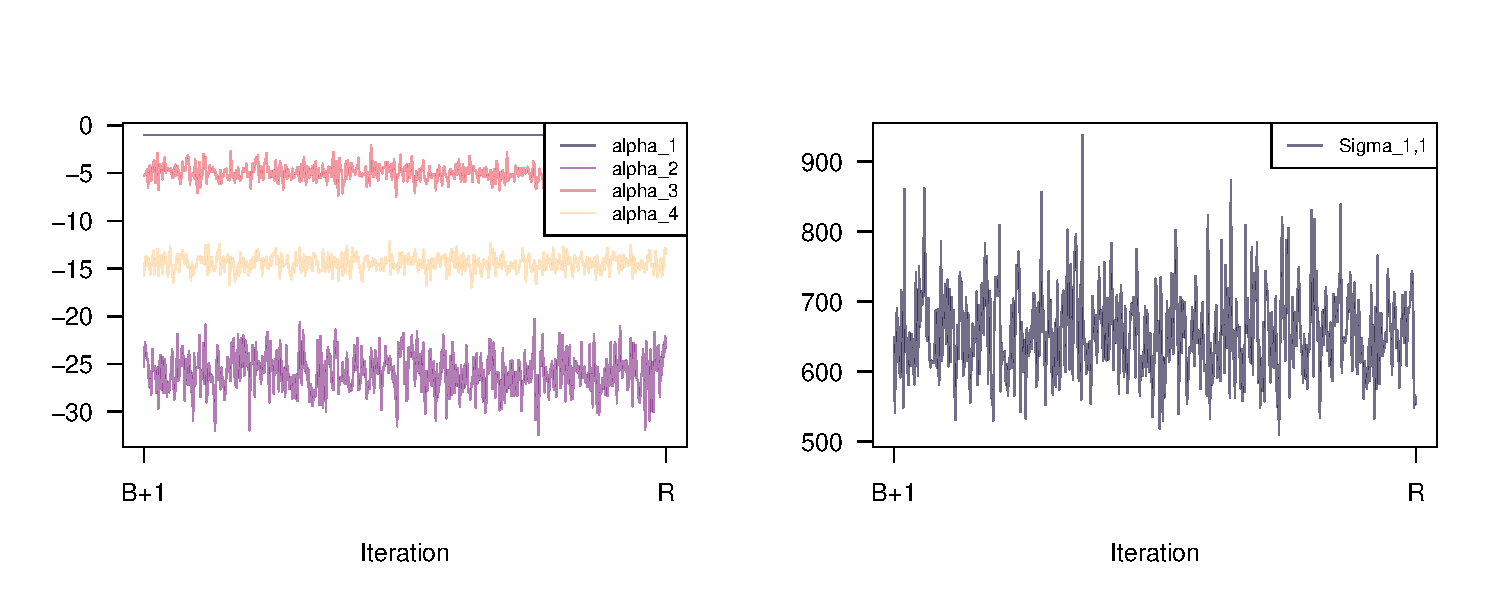
\includegraphics{rprobitb_oelschlaeger_bauer-model-train-trace}

Additionally, we can visualize the autocorrelation of the Gibbs samples via the argument \code{type = "acf"}, below exemplary for \code{alpha\_4} and \code{Sigma\_1,1}). The boxes in the plot's top-right corner state the total sample size TSS, given by (\code{R} - \code{B}) / \code{Q}, the effective sample size ESS, and the factor by which TSS is larger than ESS. The effective sample size is the value $\text{TSS} / (1 + 2\sum_{k\geq 1} \rho_k)$, where $\rho_k$ is the $k$-th order autocorrelation of the Gibbs samples \citep{Marin:2014}. The autocorrelations are estimated via the \fct{stats::acf} function.

\begin{Schunk}
\begin{Sinput}
> par(mfrow = c(1,2))
> plot(model_train, type = "acf", ignore = c("alpha_1", "alpha_2", "alpha_3"))
\end{Sinput}
\end{Schunk}
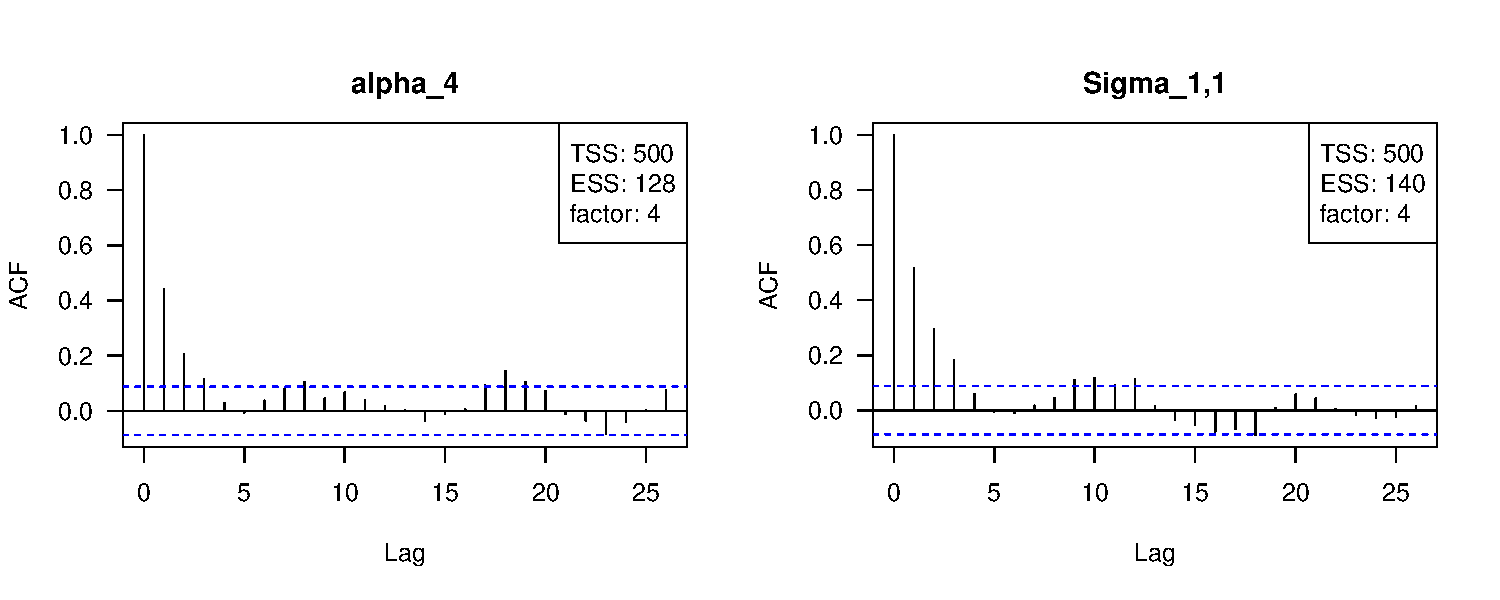
\includegraphics{rprobitb_oelschlaeger_bauer-model-train-acf}

To obtain more independent samples, the \fct{transform} method can be used to increase the thinning factor:\footnote{The function can also be used to increase the length of the burn-in period (via \code{transform(model\_train, B = B\_new)}) or to change the utility scale, for example \code{transform(model\_train, scale = "Sigma\_1 := 1")}.}

\begin{Schunk}
\begin{Sinput}
> model_train <- transform(model_train, Q = 5)
\end{Sinput}
\end{Schunk}

\subsection{Estimating a joint normal mixing distribution} \label{subsec:normal_mix}

We demonstrate how to estimate a joint normal mixing distribution in \pkg{RprobitB} on the basis of another real-data example. To enable comparison across methods and implementations, we use another data set from \pkg{mlogit}. Their results (using the logit model) are documented in the package vignette entitled "Exercise 3: Mixed logit model".

\paragraph{Example 3: Electricity suppliers.}

The \code{Electricity} data set from \pkg{mlogit} contains choices of residential electricity customers that were asked to decide between four contract offers of hypothetical electricity suppliers. Heterogeneity in choice behavior is expected here, because customers might value certain contract characteristics differently based on their living conditions. In particular, the contract offers differed in 6 characteristics: their fixed price \code{pf} per kilowatt hour, their contract length \code{cf}, whether the supplier is a local company (boolean \code{loc}), whether the supplier is a well known company (boolean \code{wk}), whether the supplier offers a time-of-day electricity price which is higher during the day and lower during the night (boolean \code{tod}), and whether the supplier's price is seasonal dependent (boolean \code{seas}).

The following lines prepare the data set for estimation. We first use the convenience function \fct{as\_cov\_names} that relabels the data columns for alternative specific covariates into the required format \code{"<covariate>\_<alternative>"}:

\begin{Schunk}
\begin{Sinput}
> data("Electricity", package = "mlogit")
> Electricity <- as_cov_names(
+    choice_data = Electricity,
+    cov = c("pf","cl","loc","wk","tod","seas"),
+    alternatives = 1:4
+  )
\end{Sinput}
\end{Schunk}

Via the \code{re = c("cl","loc","wk","tod","seas")} argument, we specify that we want to model random effects for all but the price coefficient, which we again will fix to \code{-1} to interpret the other estimates as monetary values (cf.\ Example 1):

\begin{Schunk}
\begin{Sinput}
> data_elec <- prepare_data(
+    form = choice ~ pf + cl + loc + wk + tod + seas | 0,
+    choice_data = Electricity,
+    re = c("cl","loc","wk","tod","seas")
+  )
> model_elec <- fit_model(data_elec, R = 1000, scale = "pf := -1")
\end{Sinput}
\end{Schunk}

Calling the \fct{coef} method on the estimated model returns a table of the average effects and the estimated (marginal) variances of the mixing distribution:

\begin{Schunk}
\begin{Sinput}
> coef(model_elec)
\end{Sinput}
\begin{Soutput}
        Estimate   (sd) Variance   (sd)
1   pf     -1.00 (0.00)       NA   (NA)
2   cl     -0.25 (0.03)     0.31 (0.03)
3  loc      2.79 (0.25)     7.43 (1.25)
4   wk      2.07 (0.21)     3.84 (0.67)
5  tod     -9.70 (0.21)    10.72 (1.32)
6 seas     -9.89 (0.18)     6.25 (1.03)
\end{Soutput}
\end{Schunk}

We can for example deduce, that a longer contract length has a negative effect on average (-0.25). However, our model shows that 32\% of the customers still prefer to have a longer contract length. This share is estimated by computing the proportion under the mixing distribution that yields a positive coefficient for \code{cl}:

\begin{Schunk}
\begin{Sinput}
> cl_mu <- coef(model_elec)["cl","mean"]
> cl_sd <- sqrt(coef(model_elec)["cl","var"])
> pnorm(cl_mu / cl_sd)
\end{Sinput}
\begin{Soutput}
[1] 0.3249726
\end{Soutput}
\end{Schunk}

The estimated joint mixing distribution additionally allows to infer correlations between effects. They can be extracted via the \fct{cov\_mix} function (setting \code{cor = FALSE} would return the covariances). For example, we see a correlation of 0.79 between \code{loc} and \code{wk} (deciders that prefer local suppliers also prefer well known companies):

\begin{Schunk}
\begin{Sinput}
> round(cov_mix(model_elec, cor = TRUE), 2)
\end{Sinput}
\begin{Soutput}
        cl  loc   wk   tod  seas
cl    1.00 0.09 0.07 -0.04 -0.10
loc   0.09 1.00 0.79  0.13  0.04
wk    0.07 0.79 1.00  0.14  0.03
tod  -0.04 0.13 0.14  1.00  0.55
seas -0.10 0.04 0.03  0.55  1.00
\end{Soutput}
\end{Schunk}

\subsection{Estimating a latent class model} \label{subsec:latent_classes}

\pkg{RprobitB} allows to specify a Gaussian mixture as the mixing distribution, which allows for (a) a flexible approximation of the true underlying mixing distribution and (b) a preference based classification of the deciders. To estimate such a latent mixture, pass the list \code{latent\_classes = list("C" = C)} to \fct{fit\_model}, with \code{C} being the number (greater or equal 1) of latent classes (set to 1 per default). We here assume that $C$ is known and fixed. The following Sections \ref{subsec:weight_update} and \ref{subsec:dp_update} present two updating schemes in which $C$ does not need to be pre-specified.

\paragraph{Example 2: Simulated choices (cont.).}

We previously simulated the \class{RprobitB\_data} object \code{data\_sim} from a probit model with two latent classes. We now aim to reproduce the model parameters from the data generating process:

\begin{Schunk}
\begin{Sinput}
> model_sim <- fit_model(
+    data = data_sim, R = 1000, latent_classes = list("C" = 2), seed = 1
+  )
> summary(model_sim)
\end{Sinput}
\begin{Soutput}
Probit model
Formula: choice ~ var1 | var2 | var3 
R: 1000, B: 500, Q: 1

Utility normalization
Level: Utility differences with respect to alternative 'alt2'.
Scale: Coefficient of the 1. error term variance fixed to 1.

Latent classes
C = 2 

Gibbs sample statistics
          true    mean      sd      R^
 alpha
                                      
     1   -1.00   -0.99    0.09    1.20
     2    0.00   -0.03    0.04    1.03
     3    1.00    0.93    0.09    1.07

 s
                                      
     1    0.70    0.70    0.09    1.01
     2    0.30    0.30    0.09    1.01

 b
                                      
   1.1    2.00    2.04    0.21    1.06
   1.2   -0.50   -0.51    0.28    1.00
   2.1    1.00    0.74    0.41    1.05
   2.2    1.00    1.20    0.32    1.00

 Omega
                                      
 1.1,1    0.31    0.23    0.14    1.71
 1.1,2    0.71    0.37    0.25    1.52
 1.2,2    4.67    4.33    1.16    1.04
 2.1,1    1.67    1.18    0.51    1.11
 2.1,2   -1.20   -0.71    0.35    1.03
 2.2,2    0.87    0.66    0.31    1.01

 Sigma
                                      
   1,1    1.00    1.00    0.00    1.00
\end{Soutput}
\end{Schunk}

Comparing the columns of true parameters (\code{true}) and Gibbs sample means (\code{mean}), we deduce that the model parameters (especially those characterizing the latent classes) can be estimated consistently.

\subsection{Weight-based update of the latent classes} \label{subsec:weight_update}

Adding \code{"weight_update" = TRUE} to the list for the \code{latent\_classes} argument of \fct{fit\_model} executes the following weight-based updating scheme of the latent classes (analogue to \cite{Bauer:2019}):

\begin{itemize}
  \item Class $c$ is removed, if $s_c<\varepsilon_{\text{min}}$, i.e.\ if the class weight $s_c$ drops below some threshold $\varepsilon_{\text{min}}$. This case indicates that class $c$ has a negligible impact on the mixing distribution.
  \item Class $c$ is splitted into two classes $c_1$ and $c_2$, if $s_c>\varepsilon_\text{max}$. This case indicates that class $c$ has a high influence on the mixing distribution whose approximation can potentially be improved by increasing the resolution in directions of high variance. Therefore, the class means $b_{c_1}$ and $b_{c_2}$ of the new classes $c_1$ and $c_2$ are shifted in opposite directions from the class mean $b_c$ of the old class $c$ in the direction of the highest variance.
  \item Classes $c_1$ and $c_2$ are joined to one class $c$, if $\lVert b_{c_1} - b_{c_2} \rVert<\varepsilon_{\text{distmin}}$, i.e.\ if the euclidean distance between the class means $b_{c_1}$ and $b_{c_2}$  drops below some threshold $\varepsilon_{\text{distmin}}$. This case indicates location redundancy which should be repealed. The parameters of $c$ are assigned by adding the values of $s$ from $c_1$ and $c_2$ and averaging the values for $b$ and $\Omega$.
\end{itemize}

The values for $\varepsilon_{\text{min}}$, $\varepsilon_{\text{max}}$ and $\varepsilon_{\text{distmin}}$ can be specified via the \code{latent\_classes} argument (per default \code{epsmin = 0.01}, \code{epsmax = 0.99}, and \code{distmin = 0.1}).

\paragraph{Example 2: Simulated choices (cont.).}

For our simulation example, we additionally specify \code{"C" = 10} (the initial number of latent classes) and \code{"buffer" = 5} (to execute the updating scheme only in every $buffer$-th iteration):

\begin{Schunk}
\begin{Sinput}
> model_sim <- fit_model(
+    data = data_sim, R = 1000, seed = 1,
+    latent_classes = list("C" = 10, "weight_update" = TRUE, "buffer" = 5),
+  )
\end{Sinput}
\end{Schunk}

The updating behavior of the class numbers can be visualized as follows:

\begin{Schunk}
\begin{Sinput}
> plot(model_sim, type = "class_seq")
\end{Sinput}
\end{Schunk}
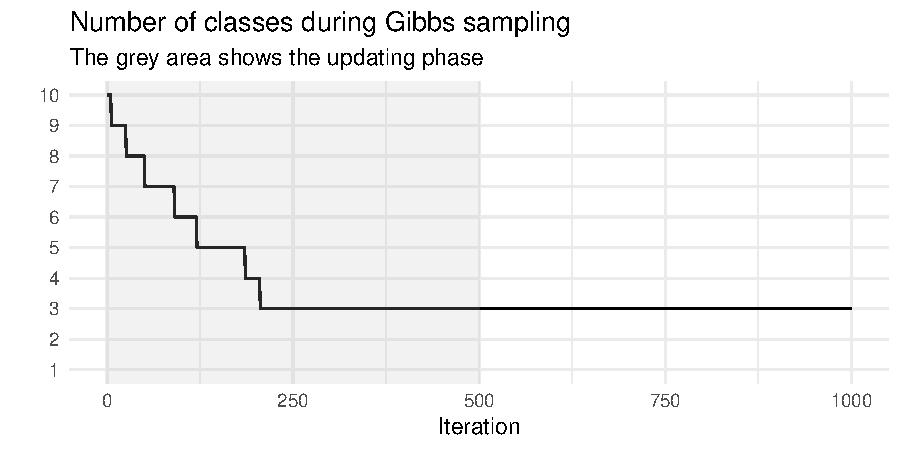
\includegraphics{rprobitb_oelschlaeger_bauer-model-sim-class-seq}

\subsection{Dirichlet process-based update of the latent classes} \label{subsec:dp_update}

The Dirichlet process is a Bayesian nonparametric method that adds as many mixture components to the mixing distribution as needed for a good approximation. We briefly formulate the theory and refer to \cite{Neal:2000} for more details.

A priori, the mixture weights $(s_c)_c$ are given a Dirichlet prior with concentration parameter $\delta/C$. For the class allocation variables $z$, \cite{Rasmussen:2000} shows that
\begin{align}
  \label{eq:all_prob}
  \Pr(z \mid \delta) = \frac{\Gamma(\delta)}{\Gamma(N+\delta)} \prod_{c=1}^C \frac{\Gamma(m_c + \delta/C)}{\Gamma(\delta/C)},
\end{align}
where $\Gamma(\cdot)$ denotes the gamma function and $m_c$ the size of class $c$. Crucially, equation \eqref{eq:all_prob} is independent of the class weights $(s_c)_c$ (in contrast to the conditional posterior distribution stated in Section \ref{subsec:prior_and_posterior}). From this equation, \cite{Li:2019} shows that
\begin{align*}
  \Pr(z_n = c \mid z_{-n}, \delta) = \frac{m_{c,-n} + \delta/C}{N-1+\delta} \to \frac{m_{c,-n}}{N-1+\delta},
\end{align*}
where the limit is taken as $C$ approaches infinity, and $z_{-n}$ denotes the vector $z$ without the $n$-th element. Now,
\begin{align*}
  1 - \sum_{c = 1}^C \frac{m_{c,-n}}{N-1+\delta} = \frac{\delta}{N-1+\delta}
\end{align*}
equals the probability that a new cluster for observation $n$ is created. This probability is directly proportional to the prior parameter $\delta$ \citep{Neal:2000}: a greater value for $\delta$ encourages the creation of new clusters, smaller values increase the probability of an allocation to an already existing class. The number of clusters can theoretically rise to infinity, however, as we delete unoccupied clusters, $C$ is bounded by $N$.

The Dirichlet process directly integrates into our existing Gibbs sampler: given $(\beta_n)_n$, we update the class means $b_c$ and covariance matrices $\Omega_c$ by means of their posterior predictive distribution. The mean vector and covariance matrix for new generated clusters are drawn from their prior predictive distribution (\cite{Li:2019} provides the formulas). The full updating scheme is implemented in the function \fct{update\_classes\_dp} and can be executed within the estimation routine \fct{fit\_model} by adding \code{dp\_update = TRUE} to the list argument for \code{latent\_classes}.

\paragraph{Example 4: Online chess strategy.}

We demonstrate the Dirichlet process updating scheme via an example from online chess. \pkg{RprobitB} containes revealed gambling preference data of chess players in the yearly bullet arena 2022 on the online chess platform https://lichess.org: at the beginning of each game, both players can choose to trade half of their clock time\footnote{Both players start a game with a time credit of one minute, which is consumend when it's their turn to make a move. A player whos time runs up looses the game automatically.} against the option to win an extra tournament point in case they win the game. The tournament lasted 4 hours, participants were paired again immediately after they finished a game, and the player with the most tournament points in the end won the event. The platform calls the trade clock time against a potential extra tournament "berserking". Several questions regarding the trade "clock time against a potential extra tournament" (which the platform calls "berserking") immediately arise: Do higher-rated chess players prefer to gamble? Does the remaining tournament time have an influence on the berserking choice? Can players be classified based on their revealed preferences to berserk?

The \code{choice\_berserk} data set provides the following information: whether a player berserked (\code{berserk = 1} if yes), wether they had the \code{white} pieces, their \code{rating} (a value provided by the platform indicating the playing strength), the rating difference \code{rating\_diff} to the opponent, whether they lost the game (\code{lost = 1} if yes), the remaining tournament time \code{min\_rem} in minutes, and whether they are currently on a winning \code{streak} (which gives extra points). We additionally consider the lagged covariates \code{berserk.1} (the berserking choice in the previous game) and \code{lost.1} (the result of a player's previous game), which can be created via the convenience function \fct{choice\_berserk}. We specify random effects for the rating difference and the result of the previous game, aiming to classify the chess players based on their berserking choice to these circumstances.

\begin{Schunk}
\begin{Sinput}
> choice_berserk <- create_lagged_cov(
+    choice_data = RprobitB::choice_berserk,
+    column = c("berserk","lost"), k = 1, id = "player_id"
+  )
> data <- prepare_data(
+    form = berserk ~ 0 | white + rating + rating_diff + min_rem + streak +
+      berserk.1 + lost.1 + 1,
+    re = c("rating_diff","lost.1"), choice_data = choice_berserk,
+    id = "player_id", idc = "game_id",
+    standardize = c("rating","rating_diff","min_rem"), impute = "zero"
+  )
> model_berserk <- fit_model(
+    data, latent_classes = list("dp_update" = TRUE, "C" = 10), R = 5000
+  )
\end{Sinput}
\end{Schunk}

Estimating this model with $N = 6174$ deciders, $T = 1$ to $177$ choice occasions and $126902$ choices in total took about 4 hours computation time. For convenience, we pre-computed the model and saved the resulting \code{model\_berserk} object in the package:

\begin{Schunk}
\begin{Sinput}
> data(model_berserk, package = "RprobitB")
> coef(model_berserk)
\end{Sinput}
\begin{Soutput}
                     Estimate   (sd) Variance   (sd)
1           white_0      0.04 (0.02)       NA   (NA)
2          rating_0      0.11 (0.01)       NA   (NA)
3         min_rem_0     -0.04 (0.01)       NA   (NA)
4          streak_0      0.27 (0.03)       NA   (NA)
5       berserk.1_0     -1.21 (0.02)       NA   (NA)
6             ASC_0      2.05 (0.03)       NA   (NA)
7  rating_diff_0 [1]    -0.10 (0.02)     0.08 (0.01)
8  rating_diff_0 [2]    -0.98 (0.06)     0.25 (0.05)
9  rating_diff_0 [3]    -1.65 (0.21)     1.72 (0.32)
10      lost.1_0 [1]     0.98 (0.09)     0.54 (0.10)
11      lost.1_0 [2]    -0.03 (0.08)     0.28 (0.06)
12      lost.1_0 [3]    -1.09 (0.18)     0.99 (0.21)
\end{Soutput}
\end{Schunk}

The classes can be visualized via calling the \fct{plot} method with the additional argument \code{type = mixture}:

\begin{Schunk}
\begin{Sinput}
> plot(model_berserk, type = "mixture")
\end{Sinput}
\end{Schunk}
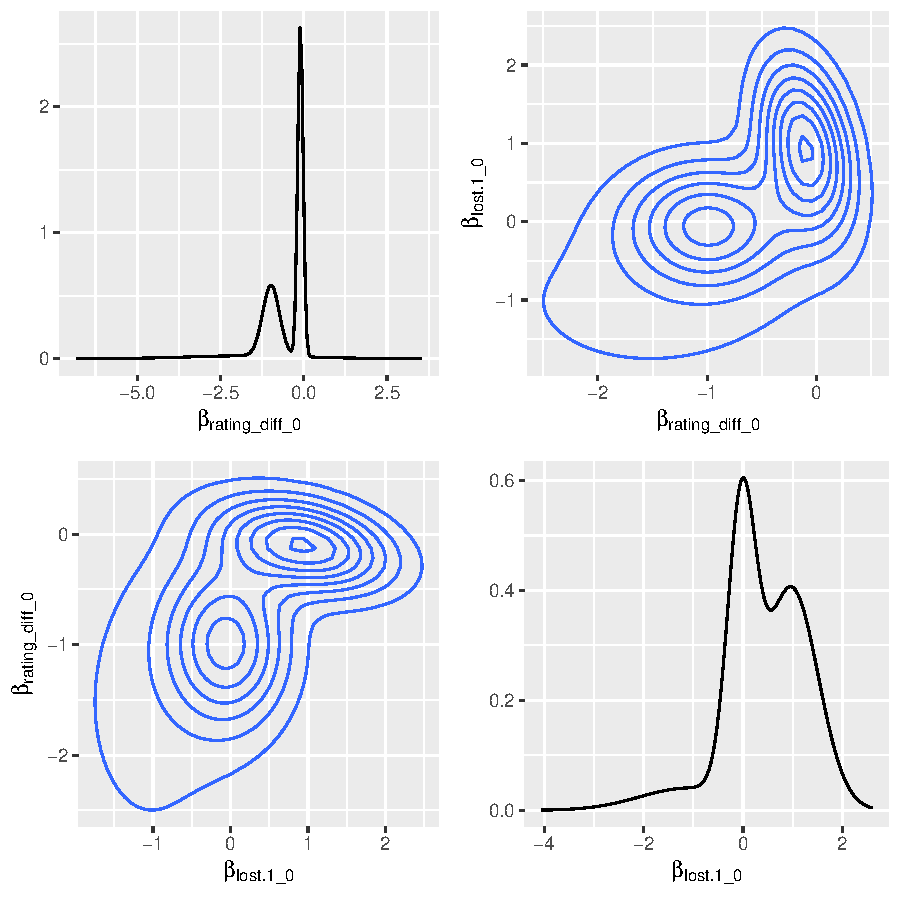
\includegraphics{rprobitb_oelschlaeger_bauer-model-berserk-mixture}

\begin{Schunk}
\begin{Sinput}
> head(preference_classification(model_berserk), n = 5)
\end{Sinput}
\begin{Soutput}
                        1     2     3 est
a_chess_player_123  0.556 0.376 0.068   1
a_nizamoff          0.276 0.648 0.076   2
a_salikhov          0.828 0.172 0.000   1
a137p314            0.616 0.368 0.016   1
a1bharadwaj2019_64k 0.684 0.296 0.020   1
\end{Soutput}
\end{Schunk}

\section{Choice prediction} \label{sec:choice_prediction}

\pkg{RprobitB} provides a \fct{predict} method for in-sample and out-of-sample prediction. The former case refers to reproducing the observed choices on the basis of the covariates and the fitted model and subsequently using the deviations between prediction and reality as an indicator for the model performance. The latter means forecasting choice behavior for changes in the choice attributes. For illustration, we revisit our probit model of travelers deciding between two fictional train route alternatives.

\paragraph{Example 1: Train trips (cont.).}

Per default, the \fct{predict} method returns a confusion matrix, which gives an overview of the in-sample prediction performance: Warning Train p. 69.

\begin{Schunk}
\begin{Sinput}
> predict(model_train)
\end{Sinput}
\begin{Soutput}
    predicted
true    A    B
   A 1034  440
   B  452 1003
\end{Soutput}
\end{Schunk}

By setting the argument \code{overview = FALSE}, the method instead returns predictions on the level of individual choice occasions:\footnote{Incorrect predictions can be analyzed via the convenience function \fct{get\_cov}, which extracts the characteristics of a particular choice situation.}

\begin{Schunk}
\begin{Sinput}
> pred <- predict(model_train, overview = FALSE)
> head(pred, n = 5)
\end{Sinput}
\begin{Soutput}
  id choiceid    A    B true predicted correct
1  1        1 0.92 0.08    A         A    TRUE
2  1        2 0.64 0.36    A         A    TRUE
3  1        3 0.79 0.21    A         A    TRUE
4  1        4 0.18 0.82    B         B    TRUE
5  1        5 0.55 0.45    B         A   FALSE
\end{Soutput}
\end{Schunk}

Apart from the prediction accuracy, the model performance can be evaluated more nuanced in terms of sensitivity and specificity, for example via a receiver operating characteristic (ROC) curve \citep{Fawcett:2006}, using the \pkg{plotROC} package \citep{Sachs:2017}:

\begin{Schunk}
\begin{Sinput}
> library(plotROC)
> ggplot(data = pred, aes(m = A, d = ifelse(true == "A", 1, 0))) +
+    geom_roc(n.cuts = 20, labels = FALSE) +
+    style_roc(theme = theme_grey)
\end{Sinput}
\end{Schunk}
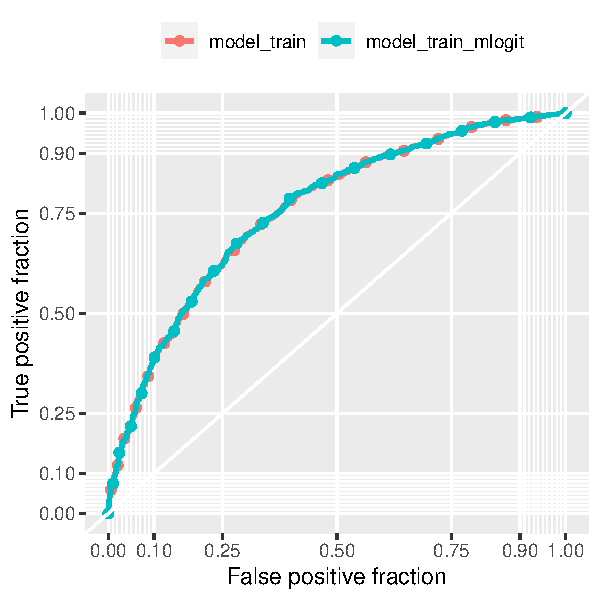
\includegraphics{rprobitb_oelschlaeger_bauer-roc-example}

The \fct{predict} method has an additional \code{data} argument. Per default, \code{data = NULL}, which results into the in-sample case outlined above. Alternatively, \code{data} can be either an \class{RprobitB\_data} object (for example a test subsample extracted via the \fct{train\_test} function) or a data frame of custom choice characteristics.

We demonstrate the second case in the following. Assume that a train company wants to anticipate the effect of a price increase on their market share. By our model, increasing the ticket price from 100 euros to 110 euros (ceteris paribus) draws 15\% of the customers to the competitor who does not increase their prices:

\begin{Schunk}
\begin{Sinput}
> predict(
+    model_train,
+    data = data.frame("price_A" = c(100,110),
+                      "price_B" = c(100,100)),
+    overview = FALSE)
\end{Sinput}
\begin{Soutput}
  id choiceid    A    B prediction
1  1        1 0.50 0.50          A
2  2        1 0.35 0.65          B
\end{Soutput}
\end{Schunk}

However, offering a better comfort class compensates for the higher price and even results in a gain of 7\% market share:

\begin{Schunk}
\begin{Sinput}
> predict(
+    model_train,
+    data = data.frame("price_A" = c(100,110), "comfort_A" = c(1,0),
+                      "price_B" = c(100,100), "comfort_B" = c(1,1)),
+    overview = FALSE)
\end{Sinput}
\begin{Soutput}
  id choiceid    A    B prediction
1  1        1 0.50 0.50          A
2  2        1 0.57 0.43          A
\end{Soutput}
\end{Schunk}

\section{Model selection} \label{sec:model_selection}

\pkg{RprobitB} provides several tools to identify the most appropriate model among competing one, including the information criteria AIC \citep{Akaike:1974}, BIC \citep{Schwarz:1978}, WAIC \citep{Watanabe:2010}, and the Bayes factor.

The WAIC is a Bayesian version of AIC and BIC and defined as $-2 \cdot \text{lppd} + 2\cdot p_\text{WAIC}$, where $\text{lppd} = \sum_i \log \left( S^{-1} \sum_s p_{si} \right)$ is the log-pointwise predictive density, $p_\text{WAIC} = \sum_i \mathbb{V}_{\theta} \log (p_{si})$ is a penalty term proportional to the variance in the posterior distribution, and $p_{si} = \Pr(y_i\mid \theta_s)$ be the probability of choice $y_i$ given the $s$-th set $\theta_s$ of parameter samples from the posterior \citep[p.\ 220]{McElreath:2016}. The $\text{WAIC}$ has a standard error of $\sqrt{n \cdot \mathbb{V}_i \left[-2 \left(\text{lppd} - \mathbb{V}_{\theta} \log (p_{si}) \right)\right]},$ where $n$ is the total number of choices. Both WAIC value and its standard error can be computed via the \fct{WAIC} method.

The Bayes factor is an index of relative posterior model plausibility of one model over another \citep{Marin:2014}: given data $y$ and two models $M_1$ and $M_2$, it is defined as
\begin{align*}
BF(M_1,M_2) = \frac{\Pr(M_1 \mid y)}{\Pr(M_2 \mid y)} = \frac{\Pr(y \mid M_1 )}{\Pr(y \mid M_2)}~/~\frac{\Pr(M_1)}{\Pr(M_2)},
\end{align*}
where per default $\Pr(M_1) = \Pr(M_2) = 0.5$. The value $\Pr(y \mid M)$ denotes the marginal model likelihood, which has no closed form and must be approximated numerically. \pkg{RprobitB} uses the posterior Gibbs samples derived from the \fct{fit\_model} function to approximate the likelihood via the posterior harmonic mean estimator \citep{Newton:1994} in combination with the prior arithmetic mean estimator \citep{Hammersley:1964}. Both estimators converge with rising posterior samples to the marginal model likelihood by the law of large numbers. Convergence is fast if the prior and posterior distribution have a similar shape and strong overlap \citep{Gronau:2017}. The estimators are implemented in the function \code{mml}. \pkg{RprobitB} provides plotting methods for analyzing the convergence behavior, see \code{help(mml, package = "RprobitB")} for details.

\paragraph{Example 1: Train trips (cont.).}

We revisit the probit model of travelers deciding between two fictional train route alternatives. As a competing model to \code{model\_train}, we consider explaining the choices only by the alternative's price, i.e.\ the probit model with the formula \code{choice ~ price | 0`}. The \fct{nested\_model} function helps in estimating such a nested model:

\begin{Schunk}
\begin{Sinput}
> model_train_sparse <- update(model_train, form = choice ~ price | 0)
\end{Sinput}
\end{Schunk}

\pkg{RprobitB} provides the convenience function \fct{model\_selection}, which takes an arbitrary number of \class{RprobitB\_fit} objects and returns a matrix of model selection criteria. The \code{criteria} input is a vector of \code{"npar"} (for the number of model parameters), \code{"LL"} (for the model's log-likelihood value, computed with the point estimates obtained from the Gibbs sample means), \code{"AIC"}, \code{"BIC"}, \code{"WAIC"}, \code{"MMLL"} (the marginal model log-likelihood), \code{"BF"} (for the Bayes factor), and \code{"pred_acc"} (the prediction accuracy). In order to compute WAIC, the marginal model likelihood, and the Bayes factor, the probabilities $p_{si} = \Pr(y_i\mid \theta_s)$ must be pre-computed via the \fct{compute\_p\_si} function:

\begin{Schunk}
\begin{Sinput}
> model_train <- compute_p_si(model_train)
> model_train_sparse <- compute_p_si(model_train_sparse)
> model_selection(
+    model_train, model_train_sparse,
+    criteria = c("npar", "LL", "AIC", "BIC", "WAIC", "MMLL", "BF", "pred_acc")
+  )
\end{Sinput}
\begin{Soutput}
                         model_train model_train_sparse
npar                               4                  1
LL                          -1727.72           -1865.86
AIC                          3463.45            3733.73
BIC                          3487.38            3739.71
WAIC                         3462.95            3734.29
se(WAIC)                        0.16               0.08
pWAIC                           3.93               1.35
MMLL                        -1730.71           -1866.89
BF(*,model_train)                  1             < 0.01
BF(*,model_train_sparse)       > 100                  1
pred_acc                      69.55%             63.40%
\end{Soutput}
\end{Schunk}

\section{Future developments} \label{sec:conclusion}

The \pkg{RprobitB} package aims at making probit models accessible to \proglang{R} users with an interest in choice behavior heterogeneity. It contains functions to prepare and simulate choice data, to fit models, to update the class size, to use a fitted model for choice prediction, and to perform model selection. The \pkg{RprobitB} package has a user-friendly design: the different package objects can be seamlessly passed between functions and its usage follows a clear workflow (see Figure \ref{fig:flowchart}). In this paper, we demonstrated for examples that serves as a starting point for \proglang{R} users who want to apply latent class mixed probit models to their own choice data.

Current limitations of the \pkg{RprobitB} package include... We plan to overcome these limitations and invite the community to suggest further features that we can implement in future package versions.

\section*{Computational details}

The results in this paper were obtained using
\proglang{R}~4.1.3 with the
\pkg{RprobitB}~1.0.0.9000 package. \proglang{R} itself
and all packages used are available from the Comprehensive
\proglang{R} Archive Network (CRAN) at \url{https://CRAN.R-project.org/}.


\section*{Acknowledgments}

This work has been financed partly by the Deutsche Forschungsgemeinschaft (DFG, German Research Foundation) - Projektnummer 356500581 which is gratefully acknowledged.

\bibliography{ref}


\end{document}
